\documentclass{article}
%% ---------------------------------------------------------------------------
%% V5 short, v0.4 (validation fold). Target venue class: PALM SHORT track
%% (hard limit 4 pp main text, excluding references and supplementary material).
%% Generated from draft.md (v0.4). Built here with tectonic in the generic
%% article class; the venue template is the NeurIPS 2026 style, which is NOT
%% installed on this machine -- the page count below is an article-class
%% approximation and must be re-measured in the venue class before freeze.
%% Swap \documentclass for the venue style at submission; keep the anonymous
%% (double-blind) build -- title/author placeholders stay blank in that build.
%% PALM's anonymization requirement extends to any supplementary or linked
%% material INCLUDING CODE: link only an anonymized snapshot.
%% ---------------------------------------------------------------------------
\usepackage[utf8]{inputenc}
\usepackage[T1]{fontenc}
\usepackage{amsmath,amssymb}
\usepackage{graphicx}
\usepackage{booktabs}
\usepackage{microtype}
\usepackage{hyperref}
\usepackage[margin=1in]{geometry}

\newcommand{\nhalf}{n_{1/2}}
\newcommand{\geff}{\gamma_{\rm eff}}
\newcommand{\Dth}{D_\theta}
\newcommand{\lth}{\ell_\theta}

\title{[WORKING TITLE: Forgetting You Can Budget, Delete and Schedule:
A $(\mu,\gamma,T)$ Law, Exact Store-Level Deletion, and a Memory Lifecycle
for a Physics-Structured Recurrent Memory]}
\author{[AUTHORS PLACEHOLDER]}
\date{}

\setlength{\emergencystretch}{3em}
\begin{document}
\maketitle

\begin{abstract}
A memory that forgets is only useful if you can say \emph{how fast}, \emph{why}, and \emph{what is actually gone}. In a physics-structured recurrent memory --- a damped symplectic (velocity-Verlet) step of a learned Hamiltonian --- forgetting is a \textbf{budget} in three numbers: the stored direction's spectral mass $\mu$, the damping $\gamma$ and the temperature $T$. The headline is a \textbf{damping optimum}: retention half-life is non-monotone in friction, one V-curve minimized at $\gamma_{\rm crit}=2\varepsilon\mu$ ($\propto\mu^{-2}$ overdamped, a mass-independent floor underdamped) spanning $\approx11$ orders of magnitude in $\mu^2$ and \textbf{generalizing from designed to emergent (learned-MLP) units, 3/3 seeds} (dim 4, hidden 64, laptop-CPU), and reproduced on a direct nonlinear rollout of the same models (argmin agreeing to $0.35\%$). Hence at $T>0$ \textbf{friction preserves and temperature erases}, and a localized friction hole is a memory vault: $107.77\pm4.78\times$ on the designed register and, law-referenced, $106.1\pm5.0\times$ on emergent units (3 seeds each) --- though the field-versus-scalar contrast that names its mechanism is designed-only. Removal is structural: under canonical placement --- Blelloch \& Golovin's (FOCS'07) --- \textbf{store-level deletion is exact}, the post-deletion store byte-identical at every load measured to the store that never held the item, under three stated conditions (\texttt{budget >= n\_cells}, \texttt{leak = 0}, priority/attribute eviction; recency eviction excluded) and on a designed store of dim 3, capacity 8--64, no learning. We ship the resulting three-state lifecycle as a mechanics demonstration, and state what decay does \emph{not} buy: \textbf{the store stops answering before it stops leaking}.
\end{abstract}

\section{Introduction}

Forgetting in a recurrent memory is a side effect --- of gate saturation, of a decaying eigenvalue, of a mixing chain --- rarely quantified in advance, and in deployed agent memories it is the failure mode benchmarks do not measure (Yang, 2026; Uddin et al., 2026). You cannot read off a trained LSTM the half-life of a stored value, the knob that sets it, or what remains once you remove it. We study a memory where all three are answerable: a damped symplectic (velocity-Verlet) step of a learnable Hamiltonian $H=T(p)+V_\theta(q)$ on $(q,p)$, where damping $p\mapsto(1-\gamma)p$ supplies forgetting, Langevin noise supplies temperature $T$, and items are optionally written as \emph{atoms}, localized wells superposed into one energy function that a dynamical relaxation reads. Our reference unit is the \textbf{CLU (Causal Learning Unit), introduced as CHLU in Jawahar \& Pierini (2026)}. Its core is exactly solvable, and we state the reduction rather than defer it: linearised at a critical point and diagonalised in the mass-whitened Hessian, one damped step acts on each normal mode as a single $2\times2$ matrix fixed by $(\varepsilon\mu,\gamma)$ alone, whose spectral radius is that mode's retention (A.0). A theory note develops the same reduction at length (Anonymous, 2026); no result here depends on it.

\textbf{Nomenclature and discipline} (full form, K.1). "Mass" names two opposed quantities: the inertial mass $M_i$ (larger $\Rightarrow$ slower) and the spectral mass $\mu_k^2=\lambda_k(M^{-1/2}\nabla^2V_\theta M^{-1/2})$ (larger $\Rightarrow$ shorter memory). Retention statements use $\mu$; a stored value lives on a near-flat coset direction; $\varepsilon$ is the integrator step, $=0.05$, never a tilt. Half-lives mean nothing without a read tolerance $\Delta$ and the thermal persistence length $\ell_\theta$, so \textbf{we never quote an $n_{1/2}$ without its $\Delta$ and $\ell_\theta/\Delta$}, and never read a designed-vs-learned distinction off raw exponents (C.5).

\textbf{Contributions.} \textbf{(1) A $(\mu,\gamma,T)$ budget with a damping optimum (\S 2.1--\S 2.2):} retention is one non-monotone V-curve minimized at $\gamma_{\rm crit}=2\varepsilon\mu$; latch, overdamped register and working memory are \textbf{three regimes of one curve, evaluated at two values of $\mu$, not two laws}, spanning $\approx11$ decades in $\mu^2$ and \textbf{generalizing to emergent (learned-MLP) units, 3/3 seeds} (dim 4, hidden 64, laptop-CPU). At $T>0$ friction preserves and temperature erases, and a friction hole is a vault whose two constituent laws hold on both arms --- $107.77\pm4.78\times$ designed, $106.1\pm5.0\times$ law-referenced on emergent, 3 seeds each --- while the field-versus-scalar contrast that names the mechanism stays designed-only. \textbf{(2) A composition, not a new deletion algorithm (\S 2.3):} the placement rule and its delete-time repair are \textbf{Blelloch \& Golovin's (FOCS'07)}; new here is composing them with a lattice packing certificate, decaying content whose decay provably commutes with deletion, and one canonical energy function read by a dynamical relaxation --- so removing an item reproduces the store holding the remaining records bit for bit, at every load from $0.29\times$ to $1.71\times$ lattice capacity and under three stated conditions; with it, the trilemma that prices lifetimes and an honest leakage statement. \textbf{(3)} A three-state memory lifecycle (PROTECTED $\rightleftarrows$ ACTIVE $\to$ TRASH, 7/7 legs), shipped as a mechanics demonstration on a toy synthetic build from which no value or benchmark number is claimed, and none was run (F).

Results on \textbf{designed testbeds} are labelled verification of exactness; on learned/emergent potentials, evidence. Every $T>0$ result requires the fluctuation--dissipation-consistent noise scale $\sigma^\star_i=\sqrt{M_iT\gamma(2-\gamma)}$ \textbf{and} a Newtonian kinetic mode (A, G). \textbf{These laws govern the store; end-to-end performance additionally depends on the encoder, measured separately, $\varphi$-bytes ledgered.}

\section{Results}

\emph{Setup (full form, A).} The step is conformally symplectic, $\det J=(1-\gamma)^d$ and $(1-\gamma\phi(q'))^d$ when position-gated, and at $T>0$ a coset random-walks with $D_\theta=\varepsilon T(2-\gamma)/(2F^2\gamma)$ (B). Checkpoints (dim 4, hidden 64, $\varepsilon=0.05$, 150 epochs) are \textbf{designed} ($SO(2)$-invariant $V_\theta$, 5 seeds) or \textbf{emergent} (MLP $V_\theta$ on identical symmetric data, 3 seeds); \S 2.3 uses the \textbf{designed atom store} (dim 3, capacity 8--64, \textbf{no learning anywhere}) (E).

\subsection{The damping optimum: one V-curve across $\approx11$ decades in $\mu^2$ (headline)}

\emph{(Designed verification + emergent evidence; provenance A.2/A.3.)}

Retention half-life is \textbf{non-monotone in friction}, and that is the organizing fact. On a trained designed-$SO(2)$ vacuum, from the model's own one-step Jacobian on a dense grid (5 seeds, dim 4), the massive radial mode's $n_{1/2}(\gamma)$ is a \textbf{V} with minimum at $\gamma_{\rm crit}=2\varepsilon\mu_{\rm rad}$ (argmin $0.076$--$0.096$ vs. predicted $0.082$--$0.116$) and log-slope $-1.006$ over $\gamma<\gamma_{\rm crit}/2$, $+1.23$--$+1.27$ over $\gamma>2\gamma_{\rm crit}$; the overdamped branch is the $\mu^{-2}$ law up to $\varepsilon\mu\approx\gamma/2$, then saturates at the mass-independent floor ($27.03$ steps at $\gamma=0.05$). The flat coset (Hessian $\mu^2\approx10^{-15}$) is the \emph{same curve at $\mu\to0$}, where $\gamma_{\rm crit}\to0$ and the register is overdamped at every $\gamma>0$: latch, overdamped register and underdamped working memory are \textbf{three regimes of one curve, evaluated at two values of $\mu$ --- not two laws}.

\textbf{This generalizes to emergent units (evidence).} On three emergent MLP checkpoints trained on identical symmetric data (dim 4, hidden 64, laptop-CPU) the coset-tracked $T=0$ half-life traces the \textbf{same V-curve}: argmin at $0.902\pm0.003\times\gamma_{\rm crit}$, log-slope $-1.0020\pm0.0003$ below and $+1.116\pm0.011$ above (fitted a factor $2.5$ either side of the minimum), \textbf{3/3 seeds}. Across both families the curve spans $\mu^2\in[1.7\times10^{-12},7\times10^{-2}]$ --- \textbf{eleven orders of magnitude} --- and the $\approx10\%$ argmin deficit is the known discrete-map correction (matched designed control $0.83$--$0.93$).

\textbf{The span's low endpoint is an instrument floor; the corner it marks has its own bound.} $1.7\times10^{-12}$ is what the ring-profile probe resolves on a designed checkpoint whose Hessian $\mu^2$ is machine zero, so eleven orders is one measured curve on one instrument. That $\mu\to0$ corner does not depend on the probe: on a direct $T=0$ rollout of five designed checkpoints (48 $\gamma$ values $\times$ 3 write amplitudes $\times$ 32 000 steps) the written angle moves by at most $9.40\times10^{-13}$ rad, so $n_{1/2}\ge9.5\times10^{15}$ steps --- a model-side bound needing no spectral instrument (C.3).

\textbf{Two instruments, one law (evidence).} Every point above is a one-step Jacobian, so we measured the same curve again by direct nonlinear rollout on the same grid, reading $n_{1/2}$ from the decay envelope's rate (3 emergent seeds, write amplitudes $0.05$--$0.5$ rad). The shape reproduces: argmin $0.9001\pm0.0052$ against $0.9032\pm0.0027$ in units of $\gamma_{\rm crit}$, log-slopes $-0.983\pm0.013$ / $+1.117\pm0.010$ against $-1.0020\pm0.0003$ / $+1.1182\pm0.0107$ on identical fit windows, and decay \emph{rates} agreeing to $0.995\pm0.003$ in the asymptotic window. What separates the instruments is a level, not a law: a first-crossing threshold reads short of the Jacobian by a per-checkpoint constant ($1.33$/$1.80$/$1.82\times$) that is flat in $\gamma$ --- coefficient of variation $2.2$--$3.7\%$ over 21--25 grid points, $|d\log\text{ratio}/d\log\gamma|\le0.0034$ --- because the ring write deposits only part of its amplitude in the slow branch (C.3). \emph{What would have falsified the law:} a stored direction that mixes normal modes, or is anharmonic at the write amplitude, has no single-mode reduction, so the curves would neither collapse nor put their minimum at $2\varepsilon\mu$. Neither happens at ten times the write amplitude: at $\delta=0.5$ rad --- the tolerance every first-passage number here uses --- the argmin moves by at most $1.4\%$, to $0.897$--$0.917\,\gamma_{\rm crit}$, and the slopes by at most $1.9\%$. The falsifier is aimed where the model information is. Below $\gamma_{\rm crit}$ the eigenpair is complex with $|\lambda|^2=1-\gamma$, an integrator identity independent of the checkpoint --- two emergent seeds differing $2.7\times$ in $\mu^2$ both print $n_{1/2}=692.5$ at $\gamma=0.002$ --- so the falsifiable content is the argmin location and the $+1$ branch, and both survive on both instruments (C.3).

\begin{figure}[t]
\centering
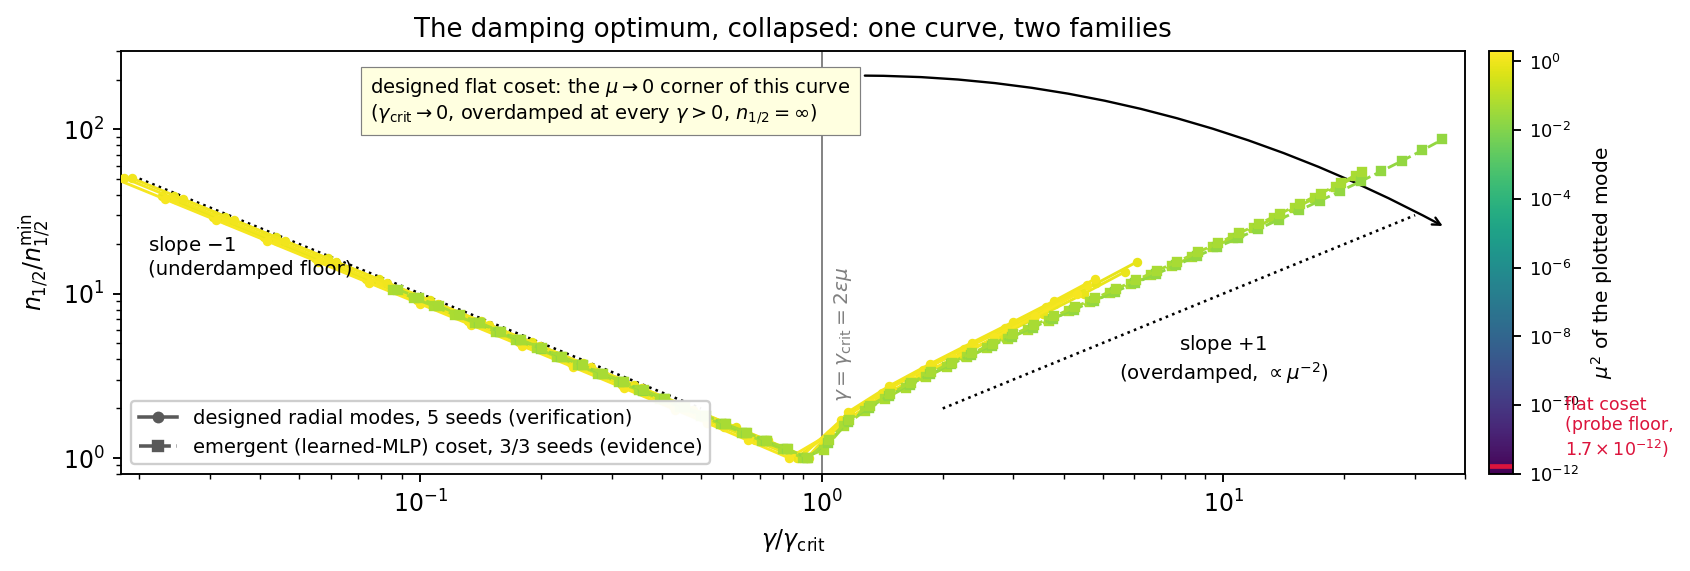
\includegraphics[width=0.70\linewidth]{figs/fig1_collapse.png}
\caption{\textbf{The damping optimum, collapsed (headline figure).} $n_{1/2}/n_{1/2}^{\min}$ against $\gamma/\gamma_{\rm crit}$, $\gamma_{\rm crit}=2\varepsilon\mu$. Eight measured curves collapse onto one: five designed radial modes (circles, verification, $\mu^2_{\rm rad}=0.670$--$1.348$) and three emergent learned-MLP coset modes (squares, evidence, $\mu^2_{\rm soft}=2.0$--$5.4\times10^{-2}$, 3/3 seeds), against the $\mp1$ asymptotes. The designed flat coset is the $\mu\to0$ corner of the same curve, marked on the colour scale at the ring-profile probe's floor $\mu^2=1.7\times10^{-12}$; that floor and the emergent $7\times10^{-2}$ are the span's endpoints (C.3). \emph{(One-step Jacobian; dim 4, hidden 64, $\varepsilon=0.05$, laptop-CPU; \texttt{langevin\_noise="fdt"}, Newtonian kinetic mode.)}}
\end{figure}

\subsection{Friction preserves, temperature erases --- and a friction hole is a vault}

\emph{(Designed verification; 5 seeds diffusion and sign flip, 3 seeds vault; A.2/A.4, B, D.)}

At $T=0$ a \textbf{designed} coset latches forever at any friction (drift $\le4.9\times10^{-12}$ rad over $200$k steps, all $\gamma\in[0.002,0.5]$, 5 seeds): friction has \textbf{zero contractive action} on a designed flat direction --- a \emph{designed-symmetry} property (below). At $T>0$ the coset decays diffusively and \textbf{raising friction slows it down}: $D_\theta=\varepsilon T(2-\gamma)/(2F^2\gamma)$ is verified to $1.0068\pm0.0219$ over 25 $(\gamma,T)$ cells, so $n_{1/2}\propto\gamma^{+1}$ and the \textbf{sign flip $\partial n_{1/2}/\partial\gamma>0$ holds in 10/10 seed$\times$temperature conditions} ($\gamma:0.05\to0.2$ \textbf{lengthens} the half-life $3.77\pm0.23\times$ at $\Delta=0.5$ rad, $\ell_\theta/\Delta<0.05$; B.3); only temperature has $\partial n_{1/2}/\partial T<0$. \emph{Fine print, beside the claim:} every $T>0$ number requires \texttt{langevin\_noise="fdt"} \textbf{and} a Newtonian kinetic mode; under the reference default these laws fail, and in the relativistic mode no noise scale targets Gibbs (G).

Hence a \textbf{memory vault}. The shipped position-gated friction field is \emph{absorb-only}, so a hole is a brake \textbf{and a refrigerator} ($T_{\rm local}=1.26\times10^{-4}$ against $10^{-3}$ outside, where a coupled bath predicts none), and the vault factor is $(\gamma_{\rm eff}/\gamma)^2$: \textbf{$107.77\pm4.78\times$} ($D_\theta$-estimator, pre-registered, 3 designed seeds, $\Delta=0.5$ rad) against $13.28\pm0.12\times$ for a \emph{scalar} friction of equal $\gamma_{\rm eff}$; the ratio $8.11\pm0.37$ is the refrigerator (D). At $T=0$ the hole erases nothing: a friction field is the wrong operator for erasing a coset (I).

\textbf{Both of the vault's laws transfer to an emergent register (evidence).} On three emergent MLP checkpoints at $T=4\times10^{-3}$ and $8\times10^{-3}$, both above the measured $T^\star$, the refrigerator law holds at $0.9998\pm0.0019$ of prediction (a $7.955\times$ refrigerator at $\gamma_\phi=0.5$ against $7.942$ predicted, the coupled-bath alternative rejected again at $0.2235$) and the $\hat D_\theta\propto\gamma_{\rm eff}^{-2}$ law at $1.016$--$1.103$, giving a law-referenced vault of $106.1\pm5.0\times$ beside the designed $107.77\pm4.78\times$. One result there has no designed analogue: \textbf{the hole confines}. The fraction of sampled states outside the register ($|\theta|>1$ rad) falls from $5.5/43.0/2.4\%$ with no hole to $0.0000$ inside it on 3/3 seeds, while a scalar friction of the same $\gamma_{\rm eff}$ still hops ($0.73/10.2/0.26\%$) --- the refrigerator turns a hopping rotor into a bounded register, and friction alone does not. \textbf{The contrast number stays designed-only:} on emergent the field/scalar ratio measures $23.39\pm10.06$ because the \emph{control} arm delocalises there ($\hat D/D_{\rm flat}=1.18$--$5.23$) while the field arm sits on the law, so $8.11\pm0.37$ is quoted as a designed quantity and the direction, not the number, is what transfers (D.7). We quote no emergent $\sigma_\theta$ ratio: above $T^\star$ that diagnostic is non-stationary on these checkpoints, its own control returning $0.459\pm0.118$ where it must return $1.000$ (D.7).

\textbf{The designed-symmetry precondition --- the boundary on everything above} \emph{(evidence; \texttt{v5-gate} R1, 3 emergent seeds + a matched designed control).} The exact $T=0$ latch is a \emph{designed} object. On an MLP potential trained on identical symmetric data the softest direction is a mid-spectrum massive mode ($1-|\lambda_{\rm coset}|\approx10^{-3}$ against the designed $\le1.1\times10^{-15}$), a written value relaxes completely, and capacity is $\approx1$--$1.6$ bits: \textbf{an emergent unit of this class has no continuous coset register; continuum flat directions must be designed in} (C.2). What survives the emergent arm is exactly the headline: the V-curve (3/3 seeds) and the sign flip above a measured $T^\star\approx3\times10^{-3}$. The same boundary bounds two extrapolations we do not make: on a \emph{learned} store the pseudo-Goldstone tilt is refuted in sign and is not a lifetime dial, the confinement capping the lifetime at $\tau_{\max}=\Gamma/2\alpha$ (K.3).

\subsection{Removal is structural: exact store-level deletion, priced lifetimes, honest leakage}

\emph{(Designed atom store, dim 3, no learning anywhere $\Rightarrow$ verification; provenance A.5--A.8, full treatment E.)}

\textbf{Stated once: external benchmarks won on their own headline metric = ZERO.} A flat table deletes exactly by construction --- the trivial substitute; at issue is a store whose items are \emph{superposed into one energy function}, where placement of one item would ordinarily depend on which others are present.

\textbf{Exact deletion, at store level.} Placement is canonical --- a function of the live records and the geometry alone --- so removing an item reproduces the store holding the remaining records bit for bit (deletion and decay provably commute; E.2). Measured: \emph{"with the waitlist, store-level deletion is exact at every load measured, $0.29\times$--$1.71\times$ lattice capacity --- AUC $0.5000\pm0.0000$ on all six statistics, byte-equal $1.0000$ --- under three stated conditions (\texttt{budget >= n\_cells}, \texttt{leak = 0}, priority/attribute-based eviction; recency-based eviction remains intrinsically history-dependent and is excluded)."} The allocator it replaces leaks membership after eviction (AUC $0.99985$ at full load, E.5), and the packing price of exactness is negative: canonical placement admits strictly more keys than the refuse-and-relocate rule it replaces (E.3). \textbf{This is a store-level guarantee only: the frozen encoder and any residue of past writes in a learned landscape are separate channels, measured separately; we do not claim certified $(\varepsilon,\delta)$ unlearning}. Without the waitlist, exactness fails at overflow (E.4).

\textbf{Attribution, in the same breath as the theorems.} \emph{Our placement rule is the \textbf{Blelloch--Golovin (FOCS'07)} stable-matching table, our Theorems 1--2 follow from theirs, and the fix-up cascade is theirs.} New here is only the composition --- packing certificate, decaying content with a proven delete/decay commutation, one canonical energy function --- whose price is negative where the general case can cost an exponential slowdown (Buchbinder--Petrank; full block, lineage and scope in E.2, K.2).

\textbf{Lifetimes are priced by a trilemma} --- exact value fidelity, amplitude-independent address hold, amplitude-independent read latency: pick two (E.6). The corner to lead with: \emph{dropping amplitude-independent latency} \textbf{is} \emph{the compute-adaptive-read dial --- a faded memory costs more integration steps to read, a physical, measurable statement a timestamped row cannot make.}

\textbf{What decay does not buy.} \textbf{The store stops answering before it stops leaking}: at the last amplitude before self-eviction ($A=0.051$) retention is $0.832$ --- placement-dependent, quoted for the controller-placed disk (E.5) --- while a query-level membership adversary sits at AUC $0.983$ and a white-box one at $1.000$; the curves never cross. Against an \emph{exact} adversary decay reduces the \textbf{effect size}, not the AUC, at any point in an item's life, so we claim no reduction in distinguishability per se (E.5). \textbf{The tighter laundering control fires:} a boolean TTL flag \emph{inside the same store} stays within $0.017$ AUC of physical decay against the exact adversary ($0.983$ vs $1.000$), separating only against a resolution-limited one (E.5). The differentiator we lead with is therefore the one needing no adversary model: \emph{decay contracts the addressing tolerance of an item, $R_{50}$ $1.146\to0.752$ ($1.52\times$), where a TTL dict's lookup radius is a constant hard step at $0.75$--$0.77$, independent of age} (E.5).

\section{Related work}

\emph{(Full discussion, K.2.)} Deployed long-term memories expire and delete by policy rather than by law: Zep invalidates contradicted edges with a timestamp instead of removing them (Rasmussen et al., 2025), Generative Agents weight recency by a $0.995$ decay factor in a ranking heuristic (Park et al., 2023), and Titans carries a learned forget gate (Behrouz et al., 2025). We benchmark against none of them; the contrast is structural. Each mechanism is a score, a flag or a learned hyperparameter where damping here carries a retention law, a read tolerance and a temperature, and each deletion is a tombstone where ours is a byte-identity --- which matters, since tombstoned vectors stay reconstructible in graph ANN indexes (Chakraborttii et al., 2026). In physics, dissipation turns type-A Nambu--Goldstone modes from propagating to diffusive (Minami \& Hidaka, 2018), and Mo (2026) proves that an exactly $G$-equivariant flow has \emph{at least} $\dim(G/\mathcal H)$ zero Lyapunov exponents --- the kinematics of protection, to which our budget is the constitutive complement, since the gap is $\mu^2$. Our placement rule is Blelloch \& Golovin's (2007), after Snyder (1977) and Naor \& Teague (2001); \emph{certified} removal is Guo et al.'s (2020) \S 2 Eq. (1), an $\varepsilon$ condition with an unnumbered $(\varepsilon,\delta)$ relaxation after it; and exact methods delete by isolation, with cost and capacity formalisms in place (Bourtoule et al. 2021; Ginart et al. 2019; Sekhari et al. 2021). \textbf{We make none of those claims}: ours is a store-level bit-exactness statement with the encoder excluded, coining no benchmark and making no cost claim.

\section{Limitations and future work}

\textbf{Limitations.} (i) \textbf{One architecture, one scale}: dim 4, hidden 64, laptop-CPU, 5 designed / 3 emergent seeds; store at dim 3 with no learning; lifecycle on a toy synthetic build. (ii) \textbf{The designed-symmetry precondition} (\S 2.2). (iii) Raw $T/\gamma$-exponents do not discriminate designed from emergent (C.5), and the \textbf{\texttt{fdt} + Newtonian scope} is mandatory for every $T>0$ number (G). (iv) \textbf{The V-curve's shape is instrument-independent, its absolute step counts are not}: a first-crossing threshold reads $1.33$--$1.82\times$ short of the linear-response Jacobian, a per-checkpoint constant offset (\S 2.1, C.3); and the emergent collapse spans only $2.7\times$ in $\mu^2$ across three seeds, so the eleven decades are one decade of emergent variation attached to the designed $\mu\to0$ corner. (v) \textbf{Deletion is store-level only}, under set-function eviction with recency eviction excluded, and \textbf{no deletion-cost claim is made} ($O(n)$ rebuild per operation; unrun). (vi) \textbf{No task-level payoff is claimed} (J). \textbf{Scale is a scope choice}: this short is sealed to laptop-scale evidence, and no larger-scale result is quoted or should be inferred. Named next: widening the emergent collapse beyond the $2.7\times$ in $\mu^2$ that three seeds span; the vault's contrast arm re-measured in the narrow window where both arms stay bounded; amortized per-delete cost vs. the flat-datastore substitute; deletion at $10^3$-item stores; deeper potentials; the \emph{temperature}-field shredder (I).

\section*{References}

\emph{(Excluded from the venue's main-text page budget. Every record below was verified against the publisher, proceedings or arXiv primary record; preprints are labelled as such.)}

\begin{itemize}
\item Agoritsas, E., Catania, G., Decelle, A., \& Seoane, B. (2023). Explaining the effects of non-convergent MCMC in the training of energy-based models. \emph{ICML}, PMLR 202:322--336. arXiv:2301.09428.
\item Andersson, A., \& Ottmann, T. (1995). New tight bounds on uniquely represented dictionaries. \emph{SIAM Journal on Computing} 24(5):1091--1103.
\item Anonymous (2026). \emph{The theory note} (exactly-solvable damped-symplectic retention theory). Anonymized for double-blind review.
\item Behrouz, A., Zhong, P., \& Mirrokni, V. (2025). Titans: Learning to memorize at test time. \emph{NeurIPS 2025}. arXiv:2501.00663.
\item Blelloch, G. E., \& Golovin, D. (2007). Strongly history-independent hashing with applications. \emph{48th IEEE Symposium on Foundations of Computer Science (FOCS)}, 272--282. doi:10.1109/FOCS.2007.36.
\item Blelloch, G. E., Golovin, D., \& Vassilevska, V. (2008). Uniquely represented data structures for computational geometry. \emph{11th Scandinavian Workshop on Algorithm Theory (SWAT)}, LNCS 5124:17--28. doi:10.1007/978-3-540-69903-3\_4.
\item Bourtoule, L., Chandrasekaran, V., Choquette-Choo, C. A., Jia, H., Travers, A., Zhang, B., Lie, D., \& Papernot, N. (2021). Machine unlearning. \emph{42nd IEEE Symposium on Security and Privacy (S\&P)}. arXiv:1912.03817.
\item Buchbinder, N., \& Petrank, E. (2003). Lower and upper bounds on obtaining history independence. \emph{CRYPTO 2003}, LNCS 2729:445--462. doi:10.1007/978-3-540-45146-4\_26. Journal version: \emph{Information and Computation} 204(2):291--337 (2006).
\item Chakraborttii, C., Garc\'ia Alvarado, J., Abdulofizova, S., \& Dwivedi, S. (2026). Ghost vectors: Soft-deleted embeddings remain reconstructible in HNSW vector databases. arXiv:2606.18497 (preprint).
\item Chen, C., Zhang, J., Zhang, Y., Zhang, L., Lyu, L., Li, Y., Gong, B., \& Yan, C. (2024). CURE4Rec: A benchmark for recommendation unlearning with deeper influence. \emph{NeurIPS 2024}. arXiv:2408.14393.
\item Chhikara, P., Khant, D., Aryan, S., Singh, T., \& Yadav, D. (2025). Mem0: Building production-ready AI agents with scalable long-term memory. arXiv:2504.19413 (preprint).
\item Coleman, S. (1973). There are no Goldstone bosons in two dimensions. \emph{Communications in Mathematical Physics} 31(4):259--264. doi:10.1007/BF01646487.
\item Decelle, A., Furtlehner, C., \& Seoane, B. (2021). Equilibrium and non-equilibrium regimes in the learning of restricted Boltzmann machines. \emph{NeurIPS 2021}. arXiv:2105.13889.
\item Di Bernardo, A., Valente, A., Mastrogiuseppe, F., \& Ostojic, S. (2025). Shaping manifolds in equivariant recurrent neural networks. arXiv:2511.04802 (preprint).
\item Du, Y., \& Mordatch, I. (2019). Implicit generation and modeling with energy based models. \emph{NeurIPS 2019}, 3603--3613. arXiv:1903.08689.
\item Fischer, A., \& Igel, C. (2010). Empirical analysis of the divergence of Gibbs-sampling-based learning algorithms for restricted Boltzmann machines. \emph{ICANN 2010}, LNCS 6354:208--217. doi:10.1007/978-3-642-15825-4\_26.
\item Fischer, A., \& Igel, C. (2011). Bounding the bias of contrastive divergence learning. \emph{Neural Computation} 23(3):664--673. doi:10.1162/NECO\_a\_00085.
\item Gell-Mann, M., Oakes, R. J., \& Renner, B. (1968). Behavior of current divergences under $SU_3\times SU_3$. \emph{Physical Review} 175(5):2195--2199. doi:10.1103/PhysRev.175.2195.
\item Ghazi, B., Kamath, P., Kumar, R., Manurangsi, P., Sekhari, A., \& Zhang, C. (2023). Ticketed learning--unlearning schemes. \emph{COLT}, PMLR 195:5110--5139. arXiv:2306.15744.
\item Ginart, A., Guan, M. Y., Valiant, G., \& Zou, J. (2019). Making AI forget you: Data deletion in machine learning. \emph{NeurIPS 2019}. arXiv:1907.05012.
\item Golubitsky, M., Stewart, I., \& Schaeffer, D. G. (1988). \emph{Singularities and Groups in Bifurcation Theory: Volume II}. Applied Mathematical Sciences 69, Springer. doi:10.1007/978-1-4612-4574-2.
\item Guo, C., Goldstein, T., Hannun, A., \& van der Maaten, L. (2020). Certified data removal from machine learning models. \emph{ICML}, PMLR 119:3832--3842. arXiv:1911.03030.
\item Hairer, E., Lubich, C., \& Wanner, G. (2006). \emph{Geometric Numerical Integration: Structure-Preserving Algorithms for Ordinary Differential Equations} (2nd ed.). Springer Series in Computational Mathematics 31.
\item Hartline, J. D., Hong, E. S., Mohr, A. E., Pentney, W. R., \& Rocke, E. (2005). Characterizing history independent data structures. \emph{Algorithmica} 42(1):57--74. doi:10.1007/s00453-004-1140-z.
\item Hidaka, Y., \& Minami, Y. (2020). Spontaneous symmetry breaking and Nambu--Goldstone modes in open classical and quantum systems. \emph{Progress of Theoretical and Experimental Physics} 2020(3):033A01. doi:10.1093/ptep/ptaa005.
\item Hinton, G. E., Dayan, P., Frey, B. J., \& Neal, R. M. (1995). The "wake-sleep" algorithm for unsupervised neural networks. \emph{Science} 268(5214):1158--1161. doi:10.1126/science.7761831.
\item Hochreiter, S., \& Schmidhuber, J. (1997). Long short-term memory. \emph{Neural Computation} 9(8):1735--1780. doi:10.1162/neco.1997.9.8.1735.
\item Iqbal, N., Keller, T. A., Song, Y., Miyato, T., \& Welling, M. (2026). Spontaneous symmetry breaking and Goldstone modes for deep information propagation. arXiv:2605.14685 (preprint).
\item Jawahar, P., \& Pierini, M. (2026). CHLU: The causal Hamiltonian learning unit as a symplectic primitive for deep learning. arXiv:2603.01768 (short paper, ICLR 2026 AI \& PDE workshop).
\item Krupa, M. (1990). Bifurcations of relative equilibria. \emph{SIAM Journal on Mathematical Analysis} 21(6):1453--1486. doi:10.1137/0521081.
\item Laguna, S., da Silva Goncalves, J., Vandenhirtz, M., Ryser, A., Cannistraci, I., \& Vogt, J. E. (2026). Rethinking machine unlearning: Models designed to forget via key deletion. arXiv:2603.15033 (preprint).
\item McLachlan, R. I., \& Perlmutter, M. (2001). Conformal Hamiltonian systems. \emph{Journal of Geometry and Physics} 39(4):276--300.
\item Mermin, N. D., \& Wagner, H. (1966). Absence of ferromagnetism or antiferromagnetism in one- or two-dimensional isotropic Heisenberg models. \emph{Physical Review Letters} 17(22):1133--1136. doi:10.1103/PhysRevLett.17.1133. Erratum: \emph{PRL} 17:1307.
\item Micciancio, D. (1997). Oblivious data structures: Applications to cryptography. \emph{29th ACM Symposium on Theory of Computing (STOC)}, 456--464. doi:10.1145/258533.258638.
\item Min, S., Gururangan, S., Wallace, E., Shi, W., Hajishirzi, H., Smith, N. A., \& Zettlemoyer, L. (2024). SILO language models: Isolating legal risk in a nonparametric datastore. \emph{ICLR 2024} (spotlight). arXiv:2308.04430.
\item Minami, Y., \& Hidaka, Y. (2018). Spontaneous symmetry breaking and Nambu-Goldstone modes in dissipative systems. \emph{Physical Review E} 97(1):012130. doi:10.1103/PhysRevE.97.012130.
\item Mo, H. H. (2026). Symmetry-protected Lyapunov neutral modes in equivariant recurrent networks. arXiv:2605.03338 (preprint; single author).
\item Munkhdalai, T., Faruqui, M., \& Gopal, S. (2024). Leave no context behind: Efficient infinite context transformers with Infini-attention. arXiv:2404.07143 (preprint).
\item Naor, M., \& Teague, V. (2001). Anti-persistence: History independent data structures. \emph{33rd ACM Symposium on Theory of Computing (STOC)}, 492--501. doi:10.1145/380752.380844.
\item Nijkamp, E., Hill, M., Han, T., Zhu, S.-C., \& Wu, Y. N. (2020). On the anatomy of MCMC-based maximum likelihood learning of energy-based models. \emph{AAAI 2020}. arXiv:1903.12370.
\item \"Ozdenizci, O., Rueckert, E., \& Legenstein, R. (2025). Privacy-aware lifelong learning. \emph{ICLR 2025}. arXiv:2505.10941.
\item Packer, C., Wooders, S., Lin, K., Fang, V., Patil, S. G., Stoica, I., \& Gonzalez, J. E. (2023). MemGPT: Towards LLMs as operating systems. arXiv:2310.08560 (preprint).
\item Park, J. S., O'Brien, J. C., Cai, C. J., Morris, M. R., Liang, P., \& Bernstein, M. S. (2023). Generative agents: Interactive simulacra of human behavior. \emph{UIST 2023}. arXiv:2304.03442.
\item Rasmussen, P., Paliychuk, P., Beauvais, T., Ryan, J., \& Chalef, D. (2025). Zep: A temporal knowledge graph architecture for agent memory. arXiv:2501.13956 (preprint).
\item Rusch, T. K., \& Mishra, S. (2021). Coupled oscillatory recurrent neural network (coRNN): An accurate and (gradient) stable architecture for learning long time dependencies. \emph{ICLR 2021}. arXiv:2010.00951.
\item Rusch, T. K., Mishra, S., Erichson, N. B., \& Mahoney, M. W. (2022). Long expressive memory for sequence modeling. \emph{ICLR 2022}. arXiv:2110.04744.
\item Sekhari, A., Acharya, J., Kamath, G., \& Suresh, A. T. (2021). Remember what you want to forget: Algorithms for machine unlearning. \emph{NeurIPS 2021}, 18075--18086. arXiv:2103.03279.
\item Shi, W., Lee, J., Huang, Y., Malladi, S., Zhao, J., Holtzman, A., Liu, D., Zettlemoyer, L., Smith, N. A., \& Zhang, C. (2025). MUSE: Machine unlearning six-way evaluation for language models. \emph{ICLR 2025}. arXiv:2407.06460.
\item Snyder, L. (1977). On uniquely representable data structures. \emph{18th IEEE Symposium on Foundations of Computer Science (FOCS)}, 142--146.
\item Sukhbaatar, S., Ju, D., Poff, S., Roller, S., Szlam, A., Weston, J., \& Fan, A. (2021). Not all memories are created equal: Learning to forget by expiring. \emph{ICML 2021}. arXiv:2105.06548.
\item Sundar, R., \& Tarjan, R. E. (1990). Unique binary search tree representations and equality-testing of sets and sequences. \emph{22nd ACM Symposium on Theory of Computing (STOC)}, 18--25.
\item Tieleman, T. (2008). Training restricted Boltzmann machines using approximations to the likelihood gradient. \emph{ICML 2008}, 1064--1071. doi:10.1145/1390156.1390290.
\item Toledo-Mar\'in, J. Q., Maiti, A., Fox, G. C., \& Melko, R. G. (2025). Exploring the energy landscape of RBMs: Reciprocal space insights into bosons, hierarchical learning and symmetry breaking. \emph{Machine Learning: Science and Technology} 6(3):035030. arXiv:2503.21536.
\item Uddin, M. N., Shubham, K., Blanco, E., Baral, C., \& Wang, G. (2026). From recall to forgetting: Benchmarking long-term memory for personalized agents. arXiv:2604.20006 (preprint).
\item Wang, B., Wang, F., Wang, P., Cong, J., Yu, Y., Yin, Y., Han, Z., \& Wei, B. (2026). Agentic unlearning: When LLM agent meets machine unlearning. arXiv:2602.17692 (preprint).
\item Wang, K., \& Zhang, C. (2026). MemLeak: Diagnosing information leaks in multimodal agent memory. arXiv:2606.29788 (preprint).
\item Yang, D. (2026). Control-plane placement shapes forgetting: An architectural study of agent memory across thirteen system configurations. arXiv:2606.15903 (preprint).
\item Zhong, W., Guo, L., Gao, Q., Ye, H., \& Wang, Y. (2024). MemoryBank: Enhancing large language models with long-term memory. \emph{AAAI 2024}. arXiv:2305.10250.
\end{itemize}




\appendix

%% ---- Supplementary material (does not count against the 4 pp limit) ----


\emph{Per our drafting policy the main text carries only the contribution arc; every corollary, robustness check, negative result and secondary instrument is written out in full below. Appendices are supplementary material and do not count against the 4 pp short-track limit.}

\section{Flag-provenance tables (per result group)}

\textbf{A.0 Setup, in full (banked from the main text at the 4 pp cut).} One dissipative velocity-Verlet step is \textbf{conformally symplectic} ($\det J=(1-\gamma)^d$; position-gated, $(1-\gamma\phi(q'))^d$), so per normal mode memory reduces to one $2\times2$ matrix ($\mu^2=k/m$). \emph{The reduction, stated here so that no result below depends on an external note.} Linearise the step about a critical point $q^\star$ of $V_\theta$ and diagonalise the mass-whitened Hessian $M^{-1/2}\nabla^2V_\theta M^{-1/2}$, whose eigenvalues are the spectral masses $\mu_k^2$. Because the damping acts on $p$ alone and the Verlet step is linear in the harmonic neighbourhood, the step block-diagonalises: mode $k$ evolves under a single real $2\times2$ matrix determined by $(\varepsilon\mu_k,\gamma)$, and that matrix's spectral radius $|\lambda_k|$ is the mode's per-step retention, with $n_{1/2}=\ln2/(1-|\lambda_k|)$. Its two eigenvalues are complex below the crossover $\varepsilon\mu\approx\gamma/2$ and real above it, meeting at an exceptional point --- which is the retention minimum $\gamma^\star\approx2\varepsilon\mu$. Hence retention is a V-curve minimized at $\gamma^\star\approx2\varepsilon\mu$, with an \textbf{overdamped register} at $n_{1/2}\propto\mu^{-2}$ (a Gell-Mann--Oakes--Renner law in spectral mass; Gell-Mann, Oakes \& Renner 1968), an \textbf{underdamped working memory} at the mass-independent envelope $2\ln2/(-\ln(1-\gamma))$, and a \textbf{latch} in the $\mu\to0$ corner; at $T>0$ a coset random-walks with $D_\theta=\varepsilon T(2-\gamma)/(2F^2\gamma)$ (B). Checkpoints (dim 4, hidden 64, $\varepsilon=0.05$, 150 epochs) come in two families: \textbf{designed} = architecturally-$SO(2)$-invariant $V_\theta$ (5 seeds); \textbf{emergent} = a generic MLP $V_\theta$ on identical symmetric data (3 seeds). \S 2.3 uses the \textbf{designed atom store} (dim 3, capacity 8--64, \textbf{no learning anywhere}) under canonical placement: each key has a hash point, a 64-bit priority and a metric probe order over a hex lattice of spacing $d_{\rm safe}=1.540$, and keys take cells in descending priority (E). Full configurations: A.

\emph{Mandatory: every training-config-sensitive result inherits its full flag set, so no cross-section contradiction can be constructed by a reviewer reproducing across sections. Reproduced from the source reports.}

\textbf{A.1 Designed \& emergent trained checkpoints (dynamics arms).} Base \texttt{ExperimentDConfig} --- dim $4$, hidden $64$, kinetic \texttt{newtonian\_learned}, \texttt{tie\_channel\_mass=True}, $\mathrm{dt}=\varepsilon=0.05$, circle $R=1.0\times256$ pts, \texttt{train\_epochs=150}, \texttt{lyapunov\_penalty="max"} ($\lambda=0.01$), training-time \texttt{langevin\_noise="legacy"} (weights trained f32). Potentials: designed \texttt{so2\_invariant} (seeds $\{42$--$46\}$, $n=5$), emergent \texttt{mlp} (seeds $\{42,43,44\}$, $n=3$). \textbf{All forgetting probes cast f32$\to$f64 (\texttt{jax\_enable\_x64}), set \texttt{langevin\_noise="fdt"} and re-tie the channel masses} (fold \texttt{tie\_channel\_mass} into \texttt{log\_mass}; $H$ bit-identical, pytree-level, no repo edit).

\textbf{A.2 Coset diffusion / sign flip / latch / designed V-curve} (\texttt{t-lever-forgetting}; \S 2.1 designed arm, \S 2.2, Appendix B). Repo \texttt{27f232f}$\to$\texttt{9bc2cf7} (code paths verified byte-identical across the move; headline cell re-run bit-identical, $\hat D=1.519788\times10^{-3}$). Checkpoints \texttt{designed150\_s\{42--46\}}, retied. \textbf{\texttt{langevin\_noise="fdt"} everywhere} (repo default \texttt{legacy}; none of these laws hold under it). \texttt{friction\_field}/\texttt{temperature\_field}=\texttt{none}; \texttt{tilt\_delta=0}, \texttt{spurion\_delta=0} (unbroken, exact Goldstone). $\varepsilon=0.05$; $\gamma$ grids $\{0.005,0.01,0.02,0.05,0.1,0.2\}$ and dense \texttt{geomspace(0.002,0.5,22)}; $T\in\{0,10^{-4},3\times10^{-4},10^{-3},3\times10^{-3},10^{-2}\}$ (exponents quoted only for $T\le3\times10^{-3}$, linear response). \textbf{$\Delta=0.5$ rad} for every $T>0$ $n_{1/2}$; deep-diffusive figures require $\ell_\theta/\Delta<0.05$. float64; seeds $42$--$46$, PRNG keys per $(\text{seed},T,\gamma)$. Env: JAX $0.9.0$, equinox $0.13.4$, numpy $2.4.1$, scipy $1.17.0$, main venv.

\textbf{A.3 Emergent-arm generalization} (\texttt{v5-gate} R1; \S 2.1 emergent arm, \S 2.2, Appendix C). Repo \texttt{d6f8bac} (FDT-inertia fix committed mid-session; \textbf{all runs use \texttt{common.retie(model)}}, under which \texttt{effective\_mass()}$\equiv$\texttt{effective\_inertia()} --- verified $\max|{\rm eff\_mass}-{\rm eff\_inertia}|=0$ on all checkpoints, so every number is invariant to the fix). Checkpoints \texttt{emergent150\_s\{42,43,44\}} (\texttt{potential\_type="mlp"}) + \texttt{designed150\_s44} (matched control). \textbf{\texttt{langevin\_noise="fdt"} everywhere}; retied; \texttt{friction\_field}/\texttt{temperature\_field}/\texttt{tilt\_delta}/\texttt{spurion\_delta} all off for coset probes. $\varepsilon=0.05$; \textbf{$\Delta=0.5$ rad}. Jacobian $\gamma$-grid \texttt{geomspace(0.002,0.5,48)}; $T$-sweep $\gamma\in\{0.01,0.05,0.2\}$, $T\in\{2,4,8,16,32\}\times10^{-3}$, $96$ walkers, cap $150000$ ($60000$ designed control); $0/45$ cells censored. float64; PRNG per $(\text{seed},T,\gamma)$. Harness cross-check: reproduces \texttt{t-lever}'s matched designed cell ($n_{1/2}=1690$ vs $1600$; $5.6\%$, within per-cell statistical error). Env as A.2.

\textbf{A.4 Friction-hole vault} (\texttt{v5-gate} R3; \S 2.2, Appendix D). Repo \texttt{d6f8bac}; \textbf{pre-registered} (predictions in \texttt{PREREG.md} before any harness ran). Checkpoints \texttt{designed150\_s\{42,43,44\}}, retied, \textbf{\texttt{langevin\_noise="fdt"}}. \texttt{FrictionField(k=1, gamma\_max=0.9, width=0.25, gate="compact", trainable=False)}, \texttt{init\_strength=}$\gamma_\phi$, \texttt{init\_radius=1.0} (localized) or $50.0$ (uniform control), centred on \texttt{Ring(0)}; \texttt{temperature\_field=none}; \texttt{tilt\_delta=spurion\_delta=0}. $\varepsilon=0.05$; scalar $\gamma=0.05$ (+ scalar control $0.525$), $\gamma_\phi\in\{0,0.1,0.2,0.3,0.5\}$; $T=10^{-3}$ (and $T=0$ for the erasure test); \textbf{$\Delta=0.5$ rad}. Ensembles: $V$ $2048$ walkers$\times40$ samples; $D$ $512\times10$ blocks; $T=0$ drift cap $400$k; direct-FPT $256$ walkers cap $400$k ($8$--$11\%$ right-censored on the inside arm --- median unbiased for censoring $<0.5$). float64; seeds $42,43,44$. Env as A.2. \emph{The absorb-only field means a friction hole locally cools the bath; documented as intended (previously undocumented) physics, not a bug.}

\textbf{A.5 Canonical placement --- theory and reference implementation} (\texttt{order-independent-placement}; Appendix E.1--E.2). Repo \texttt{63c668d} (local \texttt{main}; no tracked code touched). Harness: a standalone reference implementation (\texttt{pgcp.py}, \texttt{run\_exactness.py}, \texttt{run\_costs.py}, \texttt{run\_jax\_h7.py}) --- pure numpy float64 except the shipped-store identity check (JAX 0.9.0 / equinox 0.13.4, main venv). PREREG written before any run. Geometry: $s=0.35$, $d_{\rm safe}=4.4s=1.54$, $\alpha=0.02$, $\kappa=1.0$, $s_{\rm pay}=s$, dim $3$, \texttt{amp\_floor} $0.05$, leak $0.35$, codebook $\{\pm0.25,\pm0.75\}$, tol $=0.35\times0.5$. Seeds explicit per test ($0$, $101$, $200+n$, $300$, $4000+\text{trial}$, $500$, $600$, $9$, $777$, $2025$, $31337$, $10000+97\cdot\text{seed}$). \textbf{Training config: N/A --- no training anywhere} (no lyapunov / langevin / anchor / epoch flag in effect).

\textbf{A.6 Shipped placement + the deletion acceptance test} (\texttt{placement-landing}; Appendix E.3). Base \texttt{ff85573}; \textbf{code commit for all measurements \texttt{e2d44cd}} (controller/placement/store code identical since \texttt{1cc55cb}; one JSON records the base commit because that run's working directory was the main checkout while \texttt{PYTHONPATH} pointed at the build under test --- the code executed was the worktree's). Main venv, \textbf{JAX 0.9.0}, equinox 0.13.4. PREREG before any harness existed. Seeds $0,1,2$ $\times$ 8 targets $\times$ 128 paired worlds = 24 per-example values, \textbf{3 072 worlds per arm}. Store \texttt{AtomStorePotential(dim=3, capacity=8, alpha=0.02, s=0.35, s\_pay=s, kappa=1.0)}, \textbf{no learning anywhere}; controller \texttt{d\_safe = 4.4s = 1.540}, \texttt{budget = capacity}, \texttt{amp = 1.0}, \texttt{n\_relocation\_candidates = 400} (relocate arm), \texttt{evict\_policy="depth"} (canonical arms; LRU is a hard error at construction), \texttt{leak = 0} in the acceptance run. Geometry: $R_{\rm mia}=2.28695$ (\textbf{7 cells}) vs $R_{\rm sized}=2.68163$ (13 cells); rematch $R(64)=6.46846$ (61 cells), $\times1.05=6.79189$ (73 cells). Read (shipped, unmodified): two-phase, \texttt{dt 0.05}, \texttt{gamma\_address 0.05 x 400} $\to$ \texttt{gamma\_read 0.0 x 800}, tail $0.25$, 8 subsamples, 16 queries/item, $\sigma_\theta=0.15$, $\sigma_p=0.05$.

\textbf{A.7 Membership-adversary and lifetime instrument} (\texttt{mia-decay-measurement}; Appendix E.5). Base \texttt{63c668d}, working tree clean (analysis-only). Harness \texttt{mia\_harness.py} (+\texttt{analyze.py}, \texttt{decomp.py}, \texttt{payload\_dep.py}). PREREG \textbf{written before the harness existed}. Seeds $0,1,2$; \textbf{8 targets $\times$ 3 seeds = 24 per-example values; 128 paired IN/OUT worlds per target; 16 queries per world; 18 amplitude levels; 11 radii; 4 probe-noise levels.} Store \texttt{AtomStorePotential(dim=3, capacity=8, alpha=0.02, s=0.35, s\_pay=s, kappa=1.0)}, \textbf{no learning anywhere}; controller \texttt{d\_safe=1.540}, \texttt{n\_relocation\_candidates=400}, \texttt{budget = capacity = 8}, 1 target + 7 background; proposal disk $R=2.2869$, packing bound $8.00$. Amplitude set directly to $A$ ($\tau=\text{leak}\cdot t=-\ln A$ exact for the shipped law \texttt{amps *= exp(-leak)}, verified); \texttt{amp\_floor = 0.05} $\Rightarrow$ $\tau_{\rm evict}=\ln20=2.996$. Payload codebook \texttt{designed\_payloads(8, seed=0)}, spacing $2/7$, \texttt{payload\_tol = 0.1000} (the PREREG mis-stated the spacing as $1/7$ and tol as $0.05$; corrected here --- it loosens no criterion relative to the shipped cap). AUC convention: direction-calibrated per example, then averaged. JAX 0.9.0, main venv; runtime 1 009 s.

\textbf{A.8 Waitlist load sweep + gated-stiffness channel} (\texttt{deletion-waitlist-stiffness}; Appendix E.4/E.6). Base local \texttt{main} @ \texttt{082d095}; \textbf{code commit for all measurements \texttt{8731557}} (a later commit changes only the dtype a \emph{waitlisted} amplitude is rounded through --- provably a no-op in the default configuration used by every harness). Separate worktree; \textbf{shared virtualenv reused, JAX 0.9.0}, equinox 0.13.4. PREREG written before either harness existed. Seeds $0,1,2$ $\times$ 8 targets $\times$ 128 paired worlds = \textbf{3 072 worlds per cell} (identical draws to A.6/A.7). Store \texttt{AtomStorePotential(dim=3, capacity=max(8, offers), alpha=0.02, s=0.35, s\_pay=s, kappa=1.0)}, \textbf{no learning anywhere}. Controller (deletion arm): \texttt{d\_safe=1.540}, \texttt{budget = capacity}, \texttt{amp = 1.0}, \texttt{leak = 0}, \texttt{evict\_policy="depth"}, \texttt{placement="canonical"}, \texttt{lattice\_radius = 2.28695} $\Rightarrow$ \textbf{7 cells}; arms \texttt{waitlist=False} / \texttt{waitlist=True}. Gate arms: \texttt{payload\_gate} off / on with $g_0=0.05$ (=\texttt{amp\_floor}) and $g_0=0.005$, read length $\times1/\times2/\times4$, \texttt{payload\_eps = 1e-6}. Read as A.6 (\texttt{payload\_tol = 0.1}). Adversary, world construction, queries, statistics and the read imported \textbf{verbatim} from the A.7 harness.

\textbf{A.9 The three-state lifecycle build} (\texttt{c2w10-lifecycle-mechanics}; Appendix F). Commit \texttt{6e0c325}, base \texttt{main @ 9e0bb25}; separate worktree; \textbf{shared virtualenv reused, JAX 0.9.0}. Seeds $0,1,2$ (tests seeded per case). Rig: \texttt{CluSystem} with a learned $V_\theta$ (\texttt{DesignFreedomPotential}, rung \texttt{free\_mlp}, family \texttt{atoms}); \texttt{atom\_site\_local\_init=True}, \texttt{atom\_kernel=wendland} (cutoff 2.5), \texttt{atom\_width = 1.5 x} measured distinct-item spacing; \textbf{\texttt{addr\_dim = 12}} (higher address dimension = declared not-run). Address block: \textbf{cheap unfitted random projection, 0 fit steps}, standardisation and unit-ball scale from stream 0 only; $\varphi$ parameters on the byte ledger (484 B). Store: \texttt{capacity 72}, \texttt{budget = well\_budget = 64}, \texttt{leak 0.02}, \texttt{stage\_lifetimes=True}, \texttt{n\_atoms = 32 768}, \texttt{dim = 13}. Admission \texttt{d\_safe = 0.60 x} distinct-item spacing. Lifecycle: \texttt{h\_hi 2}, \texttt{h\_lo 1}, \texttt{window 2}, \texttt{d\_dwell 3}, \texttt{d\_demote 2}, \texttt{k\_streams 3}, \texttt{trash\_criterion last\_k\_streams}, \texttt{censoring\_guard True}, \texttt{f\_max 0.25}, \texttt{refresh\_monotonic False} (ships off). Budgets: chunk $C=8$, \texttt{offers\_per\_chunk 3}, \textbf{\texttt{write\_steps = 40}}, \texttt{read\_steps 200}, \texttt{address\_steps 100}, \texttt{read\_batch 128}. Stream: synthetic regime-switcher, schedule $(0,1,2,0,1,2)$ = 6 streams / 5 change points / 3 revisits, \texttt{n\_anchors 96}, jitter $0.02$, \texttt{n\_per\_stream 64} $\Rightarrow$ 384 instances, 48 chunks. \texttt{gamma\_phi} \textbf{on} in every lifecycle cell, off in the identity check. Wall 1 252 / 1 172 / 1 227 s per seed. \textbf{Venue discipline: this synthetic build is a mechanics instrument, never a claim venue.} Declared not-runs: the real stream, higher address dimension, merge verbs, prune-by-depth, the anytime curve, and any value / benchmark cell.

\textbf{A.10 Rollout validation of the V-curve, and the vault on emergent checkpoints} (\texttt{v5-vcurve-validation} ME-1/ME-3; \S 2.1, \S 2.2, C.3, D.7). Repo \texttt{7fcef50}, working tree clean throughout, \textbf{no tracked file touched}; \textbf{pre-registered} (predictions filed before any harness ran). Same checkpoints as A.2/A.3/A.4 (\texttt{emergent150\_s\{42,43,44\}}, \texttt{designed150\_s\{42--46\}}), retied on every load. \texttt{langevin\_noise="fdt"} everywhere (ME-1 is $T=0$, so the noise path is not exercised); $\varepsilon=0.05$; float64 (\texttt{jax\_enable\_x64}); weights cast f32$\to$f64. \textbf{ME-1:} $\gamma$ grid \texttt{geomspace(0.002,0.5,48)} --- bit-identical to the banked Jacobian grid; write amplitudes $\delta\in\{0.05,0.2,0.5\}$ rad released from rest at the ring-rotated vacuum; rollout length \texttt{n\_chunks=8000} with stride chosen so $n_{\rm total}\ge\max(20\,000,\,30\,n_{1/2}^{\rm jac})$, cap $1.024\times10^6$ steps; coset eigenpair rule $\lambda_{\rm ret}=\max\{|\lambda_j|:\text{coset overlap}\ge0.30\}$, identical to the banked harness; $\Delta=0.5$ rad for every first-passage number. \textbf{ME-3:} \texttt{FrictionField(k=1, gamma\_max=0.9, width=0.25, gate="compact", trainable=False)}, \texttt{init\_strength=}$\gamma_\phi\in\{0,0.1,0.2,0.3,0.5\}$, \texttt{init\_radius=50.0} (uniform stages) or $1.0$ (localized, first-passage), centred on \texttt{Ring(0)}; scalar $\gamma=0.05$ with a scalar control at $\gamma=0.525$ and no field; $T\in\{4\times10^{-3},8\times10^{-3}\}$ on emergent (designed cross-check at $10^{-3}$); no temperature field; \texttt{tilt\_delta=spurion\_delta=0}. Ensembles: variance $2048$ walkers $\times40$ samples; diffusion $1024$ walkers $\times4000$ lags; stationary spread $1024$ walkers, burn $20$k--$80$k; first passage $256$ walkers, caps $2\times10^5$ (outside/scalar) and $10^6$ (inside). Seeds are model seeds; PRNG keys derived per $(\text{seed},T,\gamma,\gamma_\phi)$. Env: main venv, \textbf{JAX 0.9.0}, equinox 0.13.4, numpy 2.4.1, scipy 1.17.0; macOS laptop CPU; $\approx73$ min total compute. \textbf{Estimator cross-check before use} (never trust a new harness): on \texttt{designed150\_s\{42,43,44\}} at $T=10^{-3}$ this report's estimator returns a field vault $112.58\pm1.09\times$ against the banked $107.77\pm4.78\times$, a scalar control $14.16\pm1.38\times$ against $13.28\pm0.12\times$, field/scalar $8.03\pm0.80$ against $8.11\pm0.37$, and reproduces the banked emergent Jacobian argmins bit-identically.

\section{The coset-diffusion law and the sign flip (full)}

\emph{(Source: \texttt{t-lever-forgetting} \S 2--5. Provenance A.2. Designed testbed $\Rightarrow$ verification.)}

\textbf{B.1 The estimator.} Block increments (blocks of $L=\max(500,20/\gamma)$ steps, $L\gamma\ge20$ so blocks are independent; measured lag-1 correlation of squared increments $|c_1|\le0.030$) compared against the exact finite-$N$ AR(1) partial-sum variance
\begin{equation*}
\mathrm{MSD}_\theta(N)=\frac{\varepsilon^2T}{F^2}\!\left[\frac{N(2-\gamma)}{\gamma}-\frac{2(1-\gamma)(1-(1-\gamma)^N)}{\gamma^2}\right]\to 2D_\theta\varepsilon N.
\end{equation*}
$512$ walkers $\times10$ blocks $=5120$ samples/cell (rel. SEM $\approx2.0\%$), Maxwell--Boltzmann momentum start, burn-in $\max(3000,10/\gamma)$.

\textbf{B.2 Diffusion law, 25 cells} (seed 44, $5\gamma\times5T$): $\hat D_\theta/D_\theta^{\rm pred}=1.0068\pm0.0219$ (min $0.9644$, max $1.0484$); $d\log D/d\log T=+0.998,+0.997,+0.992,+1.010,+1.006$; $d\log D/d\log\gamma$ raw $\approx-1.03$, and $-1.014,-0.980,-0.999,-1.001,-0.982$ after dividing the discrete $(2-\gamma)$ factor. Equipartition bonus: $\mathrm{RMS}(r-r^*)/\sqrt{T/(M_{\rm ch}\mu_{\rm rad}^2)}=1.0023\pm0.0100$ over 20 harmonic cells ($T\le3\times10^{-3}$).

\textbf{B.3 The sign flip.} $n_{1/2}$ = median first-passage step to $|\Delta\theta|\ge\Delta=0.5$ rad. $\partial n_{1/2}/\partial\gamma>0$ in \textbf{10/10} seed$\times T$ conditions: $d\log n_{1/2}/d\log\gamma=+0.9552\pm0.0422$ ($T=10^{-3}$, 5 seeds), $+0.6841\pm0.0480$ ($T=10^{-2}$, biased low by $\ell_\theta/\Delta$). Effect size $\gamma:0.05\to0.2$ = $3.77\pm0.23\times$ (per-seed $3.55,3.64,3.61,3.89,4.15$; ideal-coset toy $3.61$). $d\log n_{1/2}/d\log T=-0.956$ to $-0.979$ (deep-diffusive).

\textbf{B.4 Absolute law + resolution limit.} The pure-diffusion median $n_{1/2}=0.378748\,\Delta^2F^2\gamma/(\varepsilon^2T(2-\gamma))$ is the $\ell_\theta/\Delta\to0$ limit. Against an exact AR(1)-coset toy: $n_{1/2}^{\rm trained}/n_{1/2}^{\rm toy}=1.0020\pm0.0495$ over 20 cells; toy/pure-diffusion $-1=3.099(\ell_\theta/\Delta)-0.0059$. The trained coset \emph{is} the ideal flat coset; the entire excess is the boundary-layer bias of a persistent walker exiting an interval. \textbf{Never quote a raw $n_{1/2}$ without $\Delta$ and $\ell_\theta/\Delta$} --- raw ratios reach $1.257\pm0.261$; deep-diffusive $1.054\pm0.057$.

\textbf{B.5 The latch at $T=0$ (designed only).} $\big||\lambda_{\rm flat}|-1\big|\le1.7\times10^{-14}$ over \texttt{geomspace(0.002,0.5,22)}, 5 seeds; drift $\le4.9\times10^{-12}$ rad / 200k steps (30/30 cells); the $\gamma=0$ control drifts $142.7$ rad/20k (no latch). Transport law $q_\infty=q_0+\varepsilon p_0/(M\gamma)$ ratio $0.9921\pm0.0061$ (30 cells), the $0.8\%$ deficit resolved as a finite-amplitude ($\propto p_0^2$, centrifugal) \emph{write} artifact, $\to1.0000$ in linear response.

\textbf{B.6 The massive-mode V-curve (the unification).} From the one-step Jacobian on a dense $\gamma$ grid (\texttt{geomspace(0.002,0.5,22)}, 5 seeds), the massive radial mode's $n_{1/2}(\gamma)$ is non-monotone with a minimum at $\gamma_{\rm crit}=2\varepsilon\mu_{\rm rad}$ (measured $0.076$--$0.096$ vs. predicted $0.082$--$0.116$; per-seed $\mu^2_{\rm rad}=0.670,0.771,1.190,1.093,1.348$). The log-slopes are asymptotic fits: $-1.006$ over $\gamma<\gamma_{\rm crit}/2$ and $+1.23$--$+1.27$ over $\gamma>2\gamma_{\rm crit}$. The flat coset is the $\mu\to0$ corner where $\gamma_{\rm crit}\to0$.

\begin{figure}[t]
\centering
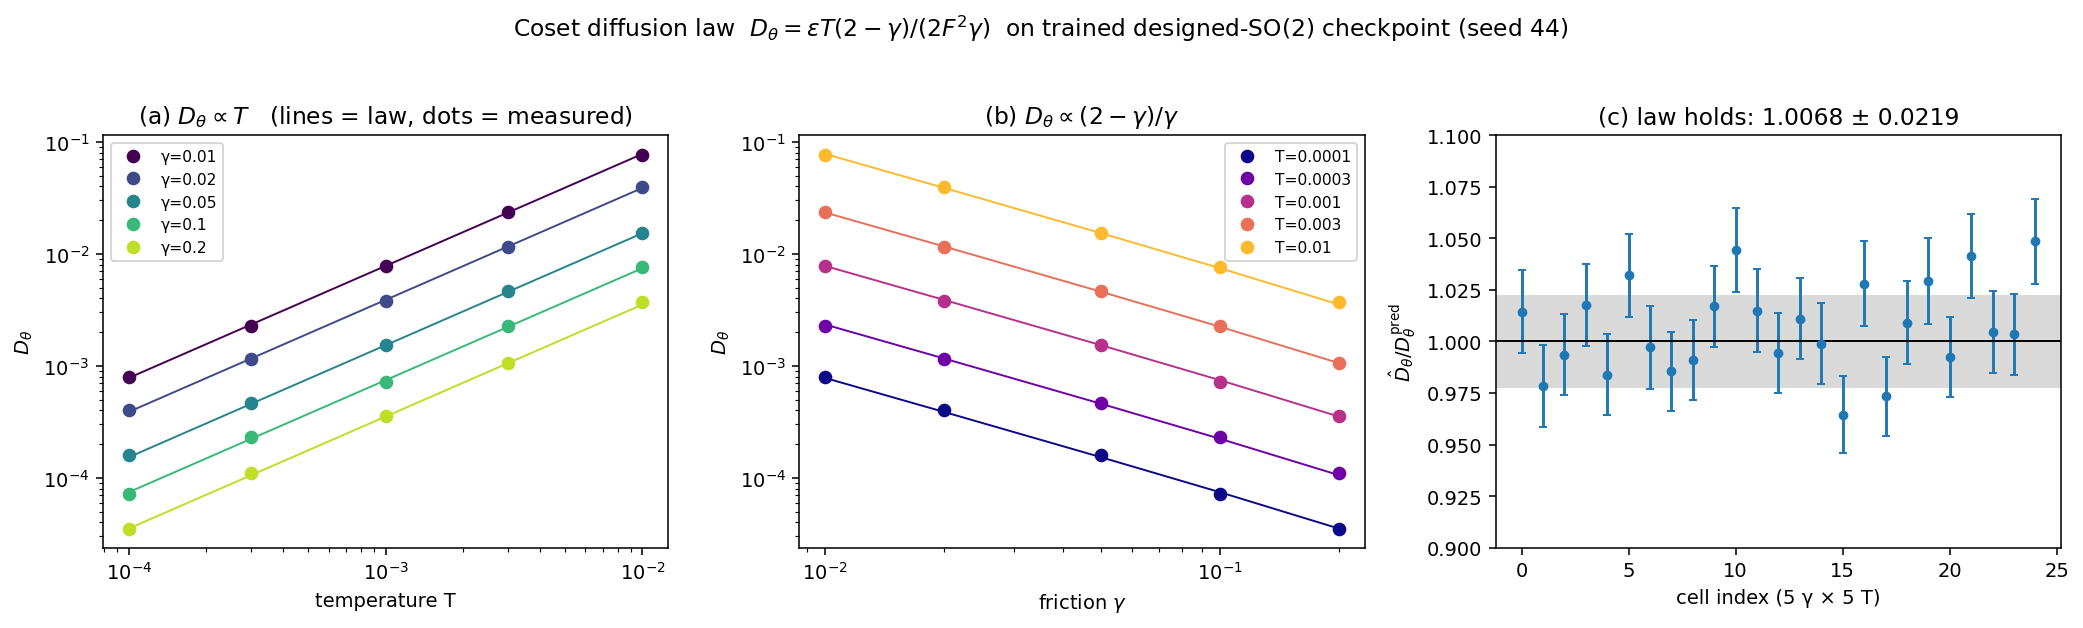
\includegraphics[width=0.70\linewidth]{figs/figB_dlaw.png}
\caption{\textbf{Figure B.1.} The coset diffusion law on a trained designed-$SO(2)$ checkpoint (seed 44): $D_\theta\propto T$, $D_\theta\propto(2-\gamma)/\gamma$, and the 25-cell ratio $\hat D_\theta/D_\theta^{\rm pred}=1.0068\pm0.0219$. \emph{(Designed testbed $\Rightarrow$ verification; \texttt{langevin\_noise="fdt"}, Newtonian kinetic mode.)}}
\end{figure}

\begin{figure}[t]
\centering
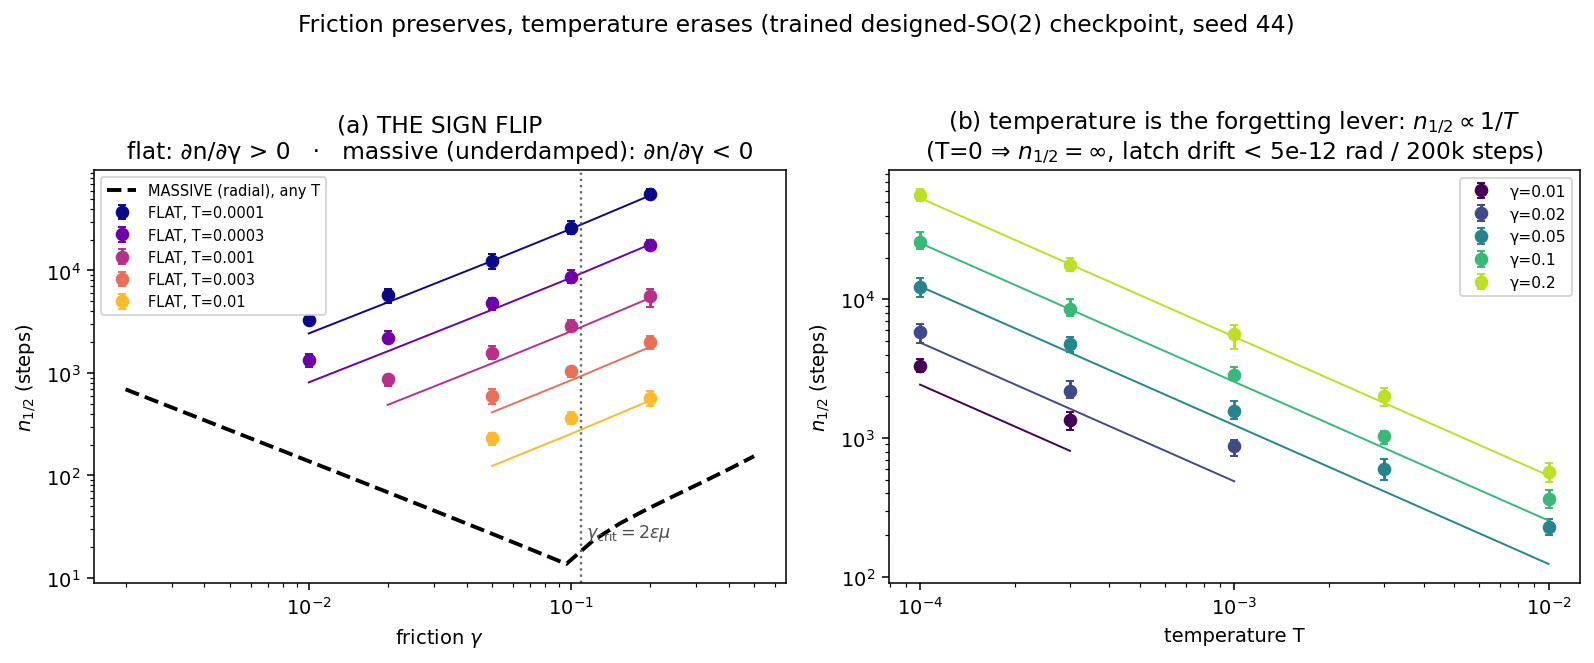
\includegraphics[width=0.70\linewidth]{figs/figB_signflip.png}
\caption{\textbf{Figure B.2.} The sign flip. Left: the flat coset's $n_{1/2}$ \emph{rises} with friction while the underdamped massive mode's falls. Right: temperature is the forgetting lever, $n_{1/2}\propto1/T$. \emph{(Designed testbed, seed 44, $\Delta=0.5$ rad $\Rightarrow$ verification.)}}
\end{figure}

\begin{figure}[t]
\centering
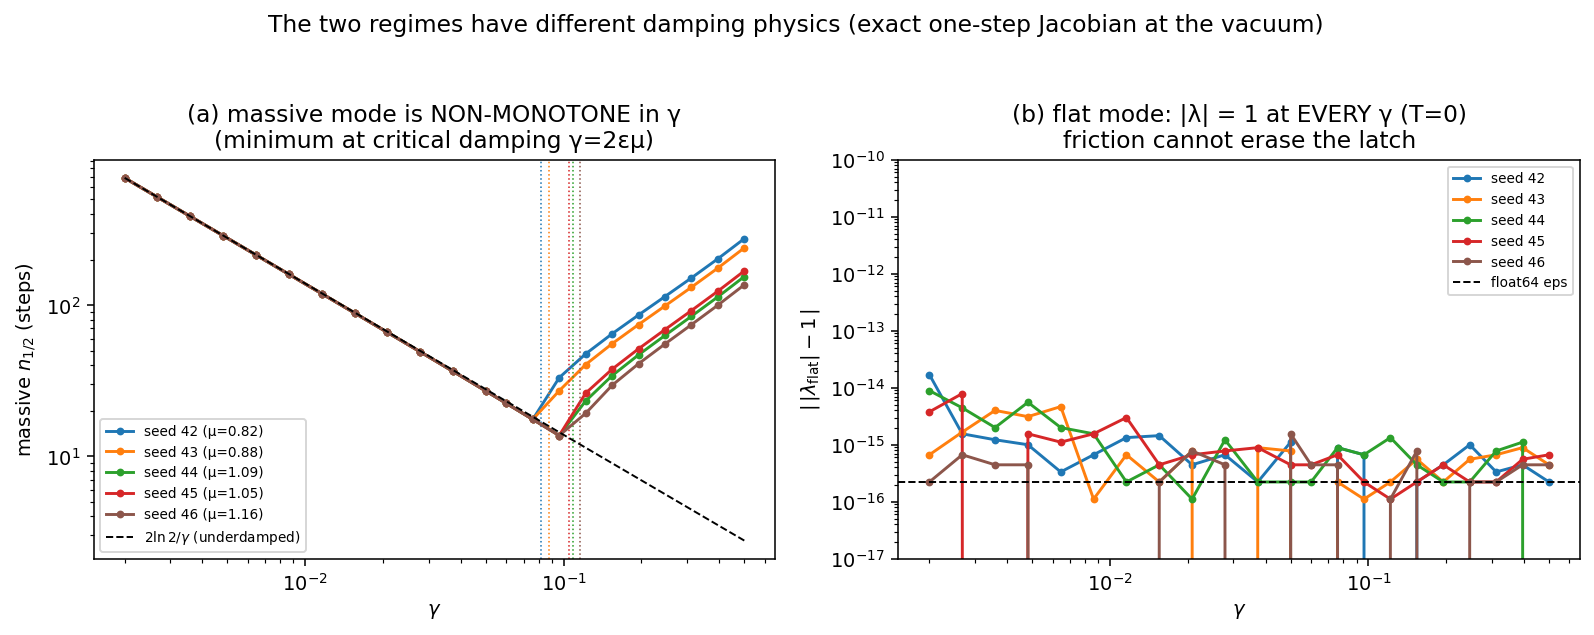
\includegraphics[width=0.70\linewidth]{figs/figB_massive_vs_flat.png}
\caption{\textbf{Figure B.3.} The two regimes, from the exact one-step Jacobian at the vacuum. Left: the massive mode is non-monotone in $\gamma$ with its minimum at $\gamma_{\rm crit}=2\varepsilon\mu$ (dotted, per seed). Right: the flat mode keeps $|\lambda|=1$ at every $\gamma$ --- friction cannot erase the latch. \emph{(Designed testbed, 5 seeds $\Rightarrow$ verification.)}}
\end{figure}

\textbf{B.7 The knob table} (all four entries measured; the $T>0$ face of the cube in one place):

\begin{table}[t]\centering\small
\begin{tabular}{p{0.307\linewidth}p{0.307\linewidth}p{0.307\linewidth}}
\toprule
stored direction & $\partial n_{1/2}/\partial\gamma$ (more friction) & $\partial n_{1/2}/\partial T$ (more heat) \\
\midrule
\textbf{coset / flat} (designed) & \textbf{$>0$} --- friction \emph{preserves} ($+0.955\pm0.042$; $3.77\times$ for $\gamma:0.05\to0.2$) & \textbf{$<0$} --- temperature \emph{erases} ($-0.956$ to $-0.979$) \\
massive (underdamped) & $<0$ --- friction shortens ($n_{1/2}$-slope $-1.006$) & $\approx0$ --- $T$ sets only the fluctuation floor $\mathrm{Var}(r-r^*)=T/(M_{\rm ch}\mu^2)$ (max/min $\le1.013$, 9/9) \\
\bottomrule
\end{tabular}
\end{table}

The coset row is the discrete analogue of the Einstein relation $D\propto T/\gamma$, and the retention consequence of the propagating$\to$diffusive transition of Minami \& Hidaka (2018/2020).

\section{The emergent arm in full (negative N46), the crossover $T^\star$, and the instrument warning}

\emph{(Source: \texttt{v5-gate} R1. Provenance A.3. Emergent-MLP $\Rightarrow$ evidence.)}

\textbf{C.1 Geometry.} Emergent coset $\mu^2_{\rm soft}=2.0\times10^{-2}$--$5.4\times10^{-2}$; stiffest/coset ratio $1.73$--$4.94$ (designed: $\infty$; $\mu^2\approx-2.9\times10^{-16}$). Washboard minima 2--3 (designed: numerically flat, 122). The emergent "flat direction" is a mid-spectrum massive mode, not a near-Goldstone.

\textbf{C.2 The latch identity fails on emergent checkpoints (the owned negative).} $1-|\lambda_{\rm coset}|=1.06\times10^{-3}$--$2.96\times10^{-3}$ at $\gamma\approx0.048$ (designed $\le1.1\times10^{-15}$; $\approx12$ orders). Over the whole $\gamma$ grid the emergent minimum is $7.6\times10^{-5}$--$2.0\times10^{-4}$ --- the more conservative figure --- against a designed grid minimum of exactly $0$. \emph{Two flatness numbers appear in this paper and they are measured on different grids:} B.5's $\big||\lambda_{\rm flat}|-1\big|\le1.7\times10^{-14}$ is the designed 22-point grid of A.2, and the $\le1.1\times10^{-15}$ quoted here is the designed control on A.3's 48-point grid. Written $\delta\in\{0.1,0.3,0.5\}$ rad relaxes completely ($|\text{retained}|\le2.1\times10^{-3}$), where designed retains $\delta$ exactly. Capacity $\log_2(2$--$3)\approx1$--$1.6$ bits, not a continuum. \textbf{An emergent unit of this class has no continuous coset register.}

\begin{figure}[t]
\centering
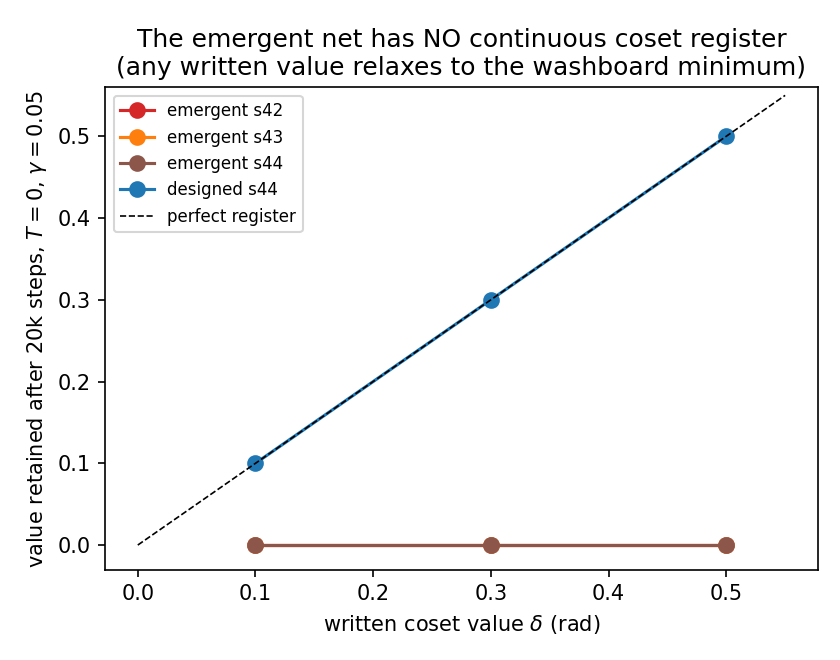
\includegraphics[width=0.70\linewidth]{figs/figC_register_capacity.png}
\caption{\textbf{Figure C.1.} The emergent unit has no continuous coset register: a written value $\delta$ relaxes to the washboard minimum at $T=0$, $\gamma=0.05$, while the designed checkpoint retains $\delta$ exactly. \emph{(Emergent MLP, 3 seeds + matched designed control $\Rightarrow$ evidence.)}}
\end{figure}

\textbf{C.3 The unification generalizes exactly --- and the instrument does not.} Emergent $T=0$ $n_{1/2}(\gamma)$ argmin$/\gamma_{\rm crit}=0.902\pm0.003$, slope $-1.0020\pm0.0003$ below / $+1.116\pm0.011$ above, 3/3 seeds, on the 48-point grid \texttt{geomspace(0.002,0.5,48)}. One curve, $\mu^2\in[1.7\times10^{-12},7\times10^{-2}]$.

\emph{Fit windows.} The designed slopes of B.6 are fitted over $\gamma<\gamma_{\rm crit}/2$ and $\gamma>2\gamma_{\rm crit}$; the emergent slopes here are fitted over $\gamma<\gamma_{\rm min}/2.5$ and $\gamma>2.5\,\gamma_{\rm min}$, with $\gamma_{\rm min}$ the parabolically refined argmin of the measured curve. Both overdamped exponents ($+1.23$--$+1.27$ designed, $+1.116\pm0.011$ emergent) exceed the continuum value $+1$ on windows of finite extent on a discrete map whose $(2-\gamma)$ factor is largest at the top of the designed grid. We do not claim the two agree, and by C.5 no designed-vs-emergent conclusion may be drawn from raw exponents in either direction.

\emph{Instrument note, so that the spans quoted in this paper cannot be read as inconsistent.} The low endpoint of the eleven-decade span, $\mu^2=1.7\times10^{-12}$, is the smallest spectral mass the Jacobian-derived ring-profile probe resolves on the designed checkpoint --- the probe validates there at ring ripple $1.9\times10^{-16}$ --- and it is not that checkpoint's Hessian $\mu^2$, which is machine zero ($|\mu^2|\approx2.9\times10^{-16}$, C.1). Eleven orders is therefore the span of one measured curve on one instrument; the $\approx12$-order designed-vs-emergent statement of C.2 is a separate quantity ($1-|\lambda_{\rm coset}|$) on a second instrument. Different instruments, same checkpoints.

\emph{The model-side replacement for that floor (provenance A.10).} The designed $\mu\to0$ corner has a bound that no spectral instrument mediates. Over 5 designed seeds $\times$ 48 $\gamma$ values $\times$ 3 write amplitudes $\times$ 32 000 steps of direct $T=0$ rollout, the worst-case departure of the written angle from its written value is $\max_n|\theta(n)-\delta|=9.400\times10^{-13}$ rad, implying a per-step rate $\Gamma\le7.309\times10^{-17}$ and $n_{1/2}\ge9.483\times10^{15}$ steps. The pre-registered bound was $10^{-6}$ rad, so this passes by about six orders of margin; the matched Hessian $\mu^2_{\rm soft}$ on those five seeds is $1.60\times10^{-15}$, $1.52\times10^{-15}$, $-2.92\times10^{-16}$, $2.94\times10^{-16}$, $1.21\times10^{-16}$. \textbf{The rollout instrument manufactures no decay at the corner}, which is the control the eleven-decade span needs and the ring-profile floor could not give.

\textbf{C.3.1 Jacobian versus rollout: the V-curve measured a second way} \emph{(provenance A.10; pre-registered; 3 emergent seeds, evidence).} Every point of the V-curve above is the one-step Jacobian's spectral gap, i.e. a linear-response quantity. We therefore ran the same $\gamma$ grid as a full nonlinear $T=0$ rollout of the trained model and compared four instruments on identical fit windows ($\gamma<\gamma_{\rm crit}/2.5$, $\gamma>2.5\gamma_{\rm crit}$, keyed to the Jacobian's $\gamma_{\rm crit}$ so the windows are not a free parameter):

\begin{itemize}
\item \textbf{I-J} --- the banked Jacobian, $n_{1/2}=\ln2/(-\ln|\lambda_{\rm ret}|)$.
\item \textbf{I-R1} --- rollout, \emph{first} crossing of $|\theta|\le\delta/2$. \textbf{This is the instrument the previously quoted disagreement was measured on.}
\item \textbf{I-R2} --- rollout, \emph{last} crossing (suffix-max envelope).
\item \textbf{I-R3 (primary)} --- rollout, envelope-\emph{rate} fit: least squares of $\log(\text{suffix-max}|\theta|)$ against $n$ over the late window $\text{env}\in[\max(10^{-6},30\times\text{floor}),\,0.3\delta]$, $n_{1/2}=\ln2/\Gamma_{\rm roll}$. Fit $R^2\ge0.9955$ (median $0.9996$) on every emergent cell.
\end{itemize}

\begin{table}[t]\centering\small
\begin{tabular}{p{0.184\linewidth}p{0.184\linewidth}p{0.184\linewidth}p{0.184\linewidth}p{0.184\linewidth}}
\toprule
checkpoint & $\gamma_{\rm crit}$ & argmin$/\gamma_{\rm crit}$ (I-J / I-R1 / I-R2 / \textbf{I-R3}) & slope below (I-J / I-R1 / I-R2 / \textbf{I-R3}) & slope above (I-J / I-R1 / I-R2 / \textbf{I-R3}) \\
\midrule
emergent seed 42 & $0.02334$ & $0.8994$ / $0.0857$ / $0.2068$ / \textbf{$0.8928$} & $-1.0023$ / $+0.0725$ / $-1.0556$ / \textbf{$-0.9651$} & $+1.1262$ / $+1.1027$ / $+1.1027$ / \textbf{$+1.1255$} \\
emergent seed 43 & $0.01424$ & $0.9046$ / $0.1404$ / $0.1404$ / \textbf{$0.9047$} & $-1.0016$ / $+0.0688$ / $+0.0688$ / \textbf{$-0.9977$} & $+1.1031$ / $+1.0889$ / $+1.0889$ / \textbf{$+1.1030$} \\
emergent seed 44 & $0.02265$ & $0.9055$ / $0.0883$ / $0.3031$ / \textbf{$0.9028$} & $-1.0022$ / $+0.0455$ / $-0.8854$ / \textbf{$-0.9854$} & $+1.1254$ / $+1.0977$ / $+1.0977$ / \textbf{$+1.1231$} \\
\textbf{mean $\pm$ sd} &  & \textbf{$0.9032\pm0.0027$} / $0.1048\pm0.0252$ / $0.2168\pm0.0668$ / \textbf{$0.9001\pm0.0052$} & \textbf{$-1.0020\pm0.0003$} / $+0.0623\pm0.0120$ / $-0.6240\pm0.4948$ / \textbf{$-0.9827\pm0.0134$} & \textbf{$+1.1182\pm0.0107$} / $+1.0964\pm0.0057$ / $+1.0964\pm0.0057$ / \textbf{$+1.1172\pm0.0101$} \\
\bottomrule
\end{tabular}
\end{table}

\textbf{The shape claims hold on the rollout.} The argmin reproduces to $0.35\%$ (pre-registered band $[0.75,1.05]$ in $\gamma_{\rm crit}$ units, 3/3 seeds) and both slopes sit inside their pre-registered bands ($[-1.20,-0.85]$, $[+0.90,+1.35]$), 3/3.

\textbf{The disagreement previously quoted is an amplitude offset on a threshold instrument, not a rate disagreement.} On the unambiguously overdamped branch ($\gamma\ge2\gamma_{\rm crit}$) the \emph{rate} ratio $\Gamma_{\rm jac}/\Gamma_{\rm R3}$ is $0.9935/1.0000/0.9948$ in the asymptotic window ($0.995\pm0.003$), while the \emph{threshold} ratio $n_{\rm jac}/n_{\rm R1}$ is $1.3307/1.7981/1.8204$ with a coefficient of variation of only $2.2$--$3.7\%$ over 21--25 $\gamma$-points and $d\log(\text{ratio})/d\log\gamma$ between $-0.0034$ and $+0.0001$ against a pre-registered falsification threshold of $0.10$. Cause, measured: the ring write deposits only a fraction of its amplitude in the slow branch (envelope-fit intercept $/\delta=0.638/0.644/0.327$), so a first crossing of $\delta/2$ fires early by a $\gamma$-independent factor. On the full (rather than asymptotic) window seed 44 reads $0.9216\pm0.0027$, $0.0004$ below the pre-registered per-point band, because that window includes the early decade where a second, faster mode is still present (early-window ratio $0.539$); the window-split diagnostic converges monotonically to $1$ as the fit moves into the asymptote. \textbf{Both threshold instruments are unusable below $\gamma_{\rm crit}$} and are recorded as such: I-R1's argmin sits at the grid edge ($0.105\pm0.025\,\gamma_{\rm crit}$) with a below-slope of $+0.0623\pm0.0120$ where the true slope is $-1$ --- the quarter-period artifact, now quantified --- and I-R2 carries an additive $\le\frac12$-period bias that diverges as the oscillation slows toward critical damping (argmin $0.217\pm0.067$, below-slope $-0.62\pm0.49$). Above $2\gamma_{\rm crit}$ the motion is monotone and $n_{\rm jac}/n_{\rm R2}=n_{\rm jac}/n_{\rm R1}$ identically. \textbf{Never quote a rollout $n_{1/2}$ from a first- or last-crossing threshold below $\gamma_{\rm crit}$.}

\textbf{Finite write amplitude (the answer to the linearization objection).} At $\delta=0.05/0.2/0.5$ rad the I-R3 argmin is $0.8928/0.9007/0.8968$ (seed 42), $0.9047/0.9045/0.9174$ (43), $0.9028/0.9037/0.9070$ (44), i.e. it moves by at most $+1.4\%$ over a $10\times$ amplitude range, and the slopes move by at most $1.9\%$. Every $\delta=0.5$ write relaxed all the way home ($|\theta_{\rm final}|\le6.5\times10^{-10}$), so no seed's $0.5$-rad write cleared its washboard barrier. The pre-registered early-window clause \textbf{fails}: $\Gamma_{\rm jac}/\Gamma^{\rm early}_{\rm roll}=0.52$--$0.85$ against a band of $[0.65,1.35]$, i.e. the first half-decade of decay runs up to $1.9\times$ faster than linear response. The amplitude sweep identifies that as mode mixing rather than anharmonicity --- for seed 44 the early ratio is $0.539/0.527/0.522$ across the $10\times$ amplitude range, i.e. amplitude-independent.

\textbf{What the left branch does and does not contain.} For $\gamma<\gamma_{\rm crit}$ the coset eigenpair is complex with $|\lambda|^2=1-\gamma$, so $n_{1/2}=\ln2/(-\frac12\ln(1-\gamma))$ \emph{independently of $\mu^2$ and of the checkpoint}: at $\gamma=0.002$, emergent seeds 42 ($\mu^2=5.449\times10^{-2}$) and 43 ($\mu^2=2.029\times10^{-2}$) both print $\lambda_{\rm ret}=0.998999499$ and $n_{1/2}=692.5$, against $2\ln2/0.002=693.1$. The left branch is an integrator identity; all model-dependent content of the V-curve is the argmin location $\gamma_{\rm crit}=2\varepsilon\mu$ and the $+1$ branch. What the rollout adds is that the \emph{nonlinear} model obeys that identity, which was not guaranteed.

\textbf{The collapse, on both instruments.} In collapsed variables $x=\gamma/\gamma_{\rm crit}$, $y=n_{1/2}\gamma_{\rm crit}$ on a common $x\in[0.15,20]$ grid, the three emergent curves agree to a median $1.15\%$ (max $11.09\%$) on I-J and a median $5.67\%$ (max $10.51\%$) on I-R3, the residual concentrated near the minimum where a parabolic argmin is least well conditioned. Per-seed $y_{\min}=1.579/1.527/1.499$ (I-J) and $1.631/1.535/1.662$ (I-R3) sit $22$--$24\%$ below the continuum value $2\sqrt2\ln2=1.961$, and $x_{\min}\approx0.90$ sits $27\%$ above the continuum $0.707$ --- both are the known discrete-map corrections, and the matched designed control gives $x_{\min}=0.83$--$0.93$. \textbf{Scope, stated plainly:} across the three emergent seeds $\mu^2_{\rm soft}$ spans only $2.029\times10^{-2}$--$5.449\times10^{-2}$, a factor $2.7$. The eleven-decade span is one decade of emergent variation attached to the designed $\mu\to0$ corner, and the rollout does not widen it --- it certifies that the corner is real (above).

\begin{figure}[t]
\centering
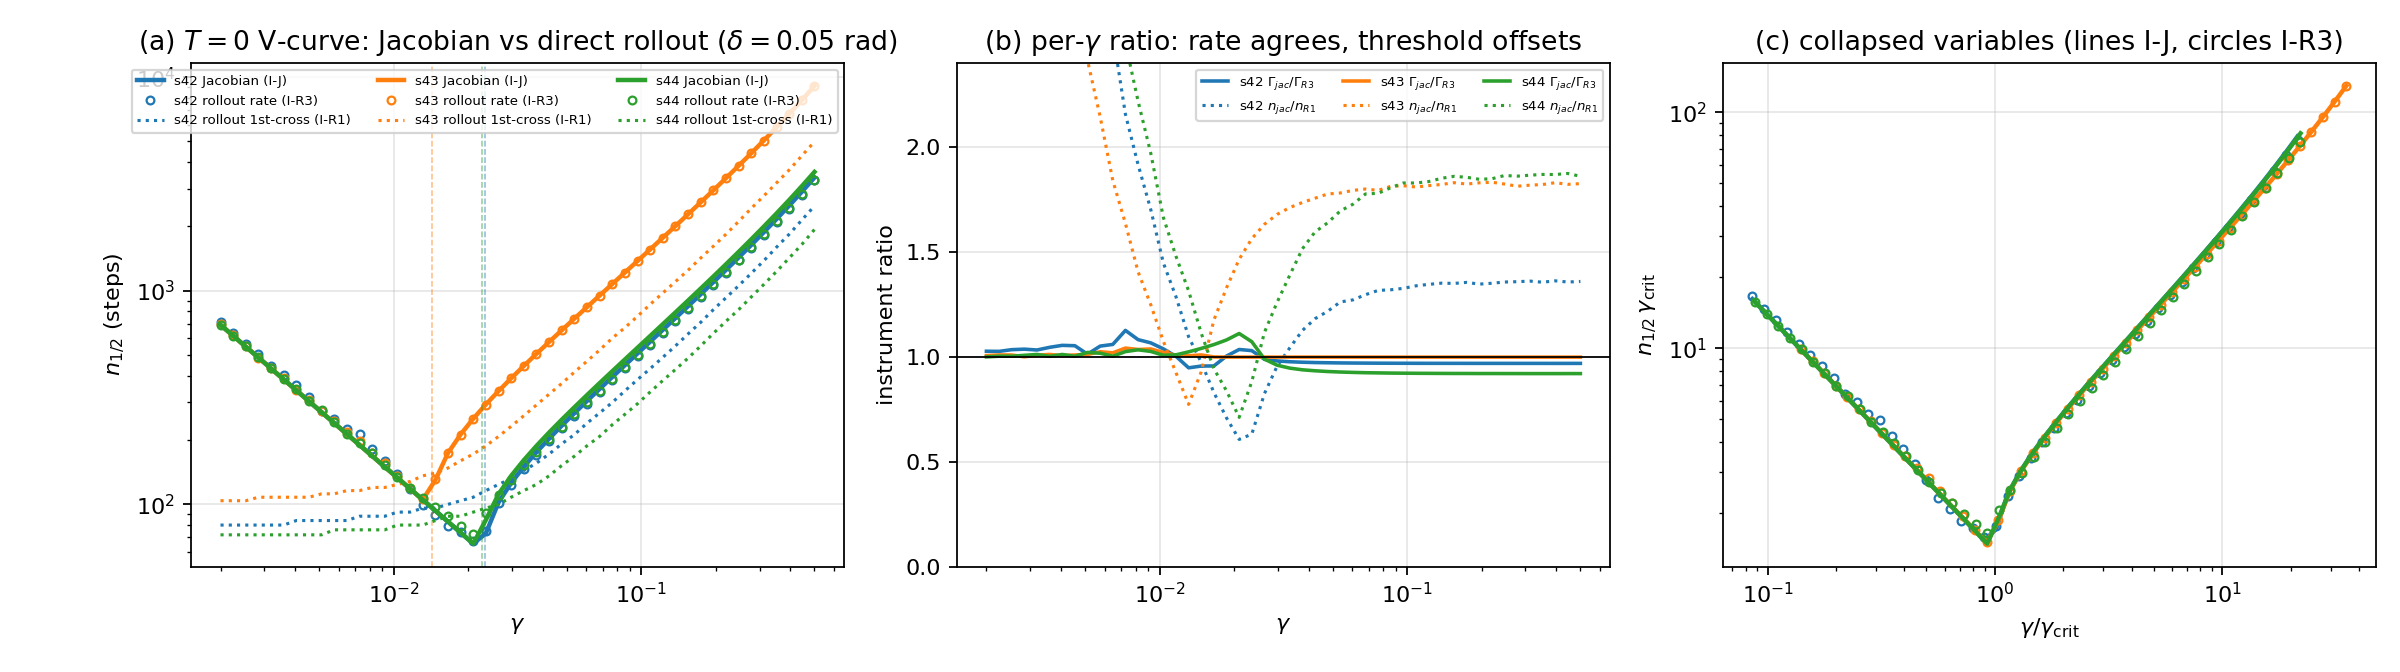
\includegraphics[width=0.70\linewidth]{figs/figC_rollout.png}
\caption{\textbf{Figure C.2.} The V-curve on two instruments. (a) $T=0$ $n_{1/2}(\gamma)$ per emergent seed: the one-step Jacobian (I-J, lines), the rollout envelope-rate instrument (I-R3, circles) and the rollout first-crossing threshold (I-R1, dotted), at write amplitude $\delta=0.05$ rad. (b) The per-$\gamma$ instrument ratio: the rate ratio $\Gamma_{\rm jac}/\Gamma_{\rm R3}$ sits on $1$, while the threshold ratio $n_{\rm jac}/n_{\rm R1}$ is offset and flat in $\gamma$ above $\gamma_{\rm crit}$. (c) The same data in collapsed variables. \emph{(Emergent MLP, 3 seeds, dim 4, hidden 64, $\varepsilon=0.05$, laptop-CPU, float64, $T=0$ $\Rightarrow$ evidence; provenance A.10.)}}
\end{figure}

\textbf{C.4 The $T>0$ face and the crossover $T^\star$.} $\partial n_{1/2}/\partial\gamma>0$ in 10/10 emergent conditions. Bias-corrected $n_{1/2}^{\rm obs}/n_{1/2}^{\rm Goldstone}$ ($\gamma=0.2$, $\ell_\theta/\Delta<0.06$): $2.75,3.40$ at $T=2\times10^{-3}$ $\to$ $0.94$--$1.25$ at $T\ge4\times10^{-3}$. \textbf{$T^\star\approx3\times10^{-3}$} (predicted $2.72$--$3.66\times10^{-3}$), comfortably below the washboard barrier ($2.29$--$3.57\times10^{-2}$). Below $T^\star$ the pseudo-Goldstone mass \emph{protects} the register; above it the emergent coset obeys the exact-Goldstone law to $\pm25\%$.

\begin{figure}[t]
\centering
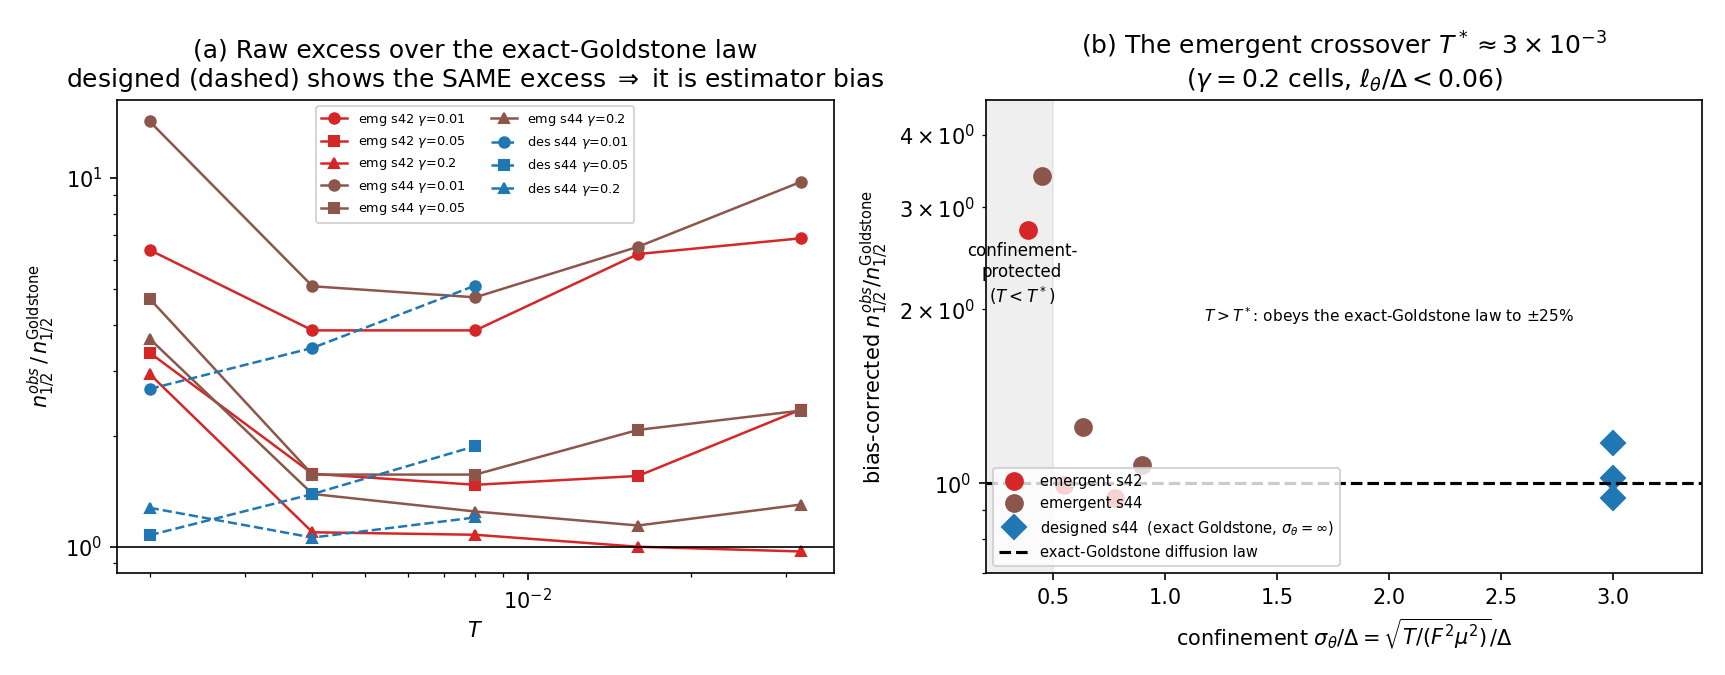
\includegraphics[width=0.70\linewidth]{figs/figC_Tstar.png}
\caption{\textbf{Figure C.3.} The crossover $T^\star$. Left: the raw excess over the exact-Goldstone law is the same on the matched designed control, so it is estimator bias, not physics. Right: bias-corrected, the emergent coset joins the exact-Goldstone law above $T^\star\approx3\times10^{-3}$. \emph{(Emergent MLP + matched designed control $\Rightarrow$ evidence; $\Delta=0.5$ rad, $\ell_\theta/\Delta<0.06$, \texttt{fdt} noise, Newtonian kinetic mode.)}}
\end{figure}

\begin{figure}[t]
\centering
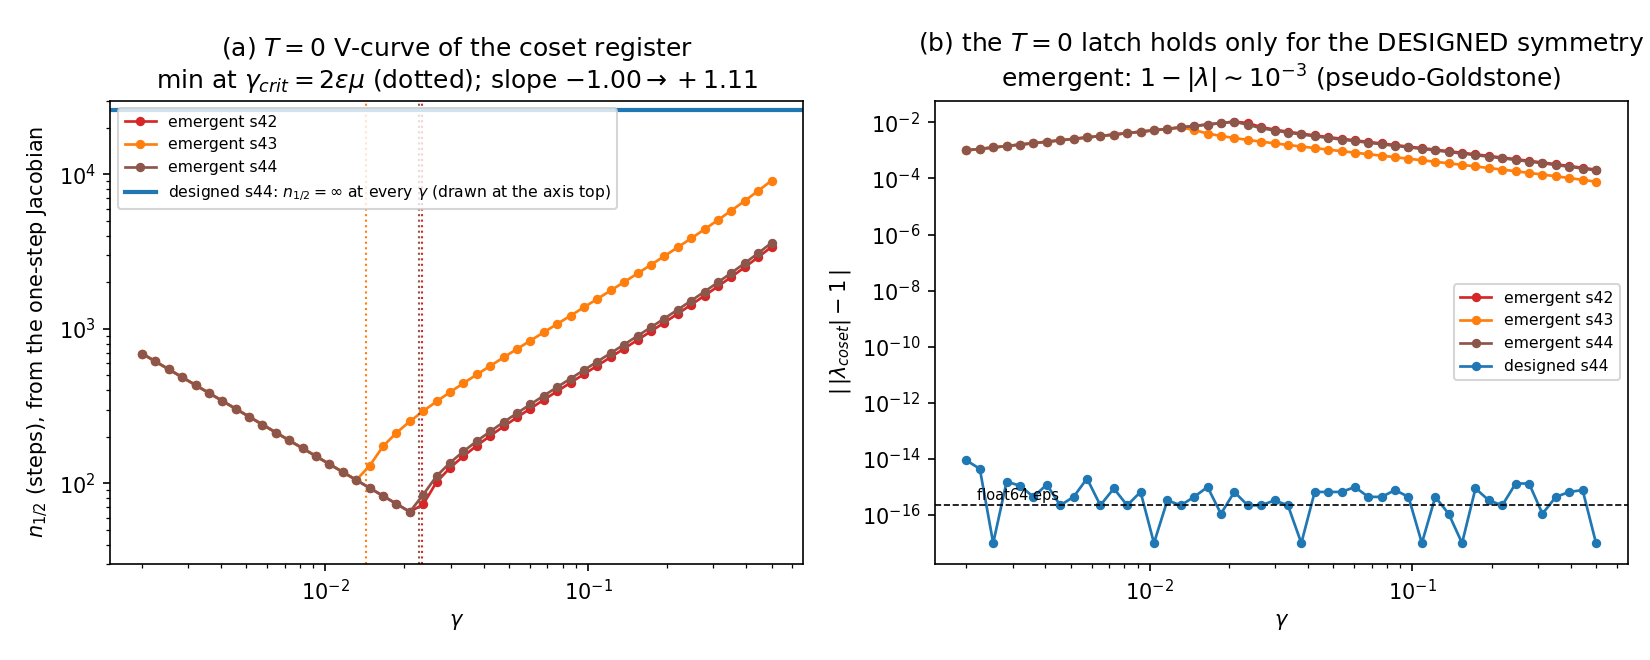
\includegraphics[width=0.70\linewidth]{figs/figC_lambda_coset.png}
\caption{\textbf{Figure C.4.} The un-collapsed form of Figure 1, and the negative beside it. Left: the emergent $T=0$ V-curve per seed, with $\gamma_{\rm crit}=2\varepsilon\mu_{\rm soft}$ dotted; the designed coset has $n_{1/2}=\infty$ at every $\gamma$ and is drawn at the axis top. Right: $\big||\lambda_{\rm coset}|-1\big|$ --- the $T=0$ latch is exact for the designed symmetry and fails by $\sim10^{-3}$ on every emergent seed. \emph{(Emergent MLP, 3 seeds + matched designed control $\Rightarrow$ evidence.)}}
\end{figure}

\textbf{C.5 The instrument warning (the most important methodological caveat in the paper).} Raw exponents are \textbf{not} discriminating: a matched designed control on the same grid gives $d\log n_{1/2}/d\log T=-0.53,-0.60,-1.04$ and $d\log n_{1/2}/d\log\gamma=+0.78,+0.63,+0.55$ --- indistinguishable from emergent, because both families carry the $\ell_\theta/\Delta$ boundary layer (reaching $\ell_\theta/\Delta=2.03$ on that grid). Only the operator $|\lambda_{\rm coset}|$ (a 12-order separation) and bias-corrected deep-diffusive cells discriminate. \textbf{Any designed-vs-emergent claim read off raw exponents is an artifact.}

\textbf{C.6 Two-observables caveat (a falsification of our own prediction).} A register written \emph{at} the washboard minimum has $\partial n_{1/2}/\partial\gamma>0$ (relaxation protects, both channels); a register written \emph{off} the minimum follows the V-curve's $\gamma<\gamma_{\rm crit}$ branch, $\partial n_{1/2}/\partial\gamma<0$. Both signs exist on the same emergent checkpoint for different observables --- the task's own prediction that the slope "flips back to negative below $T^\star$" is refuted and structurally cannot hold for a register written at the vacuum. \textbf{A "sign flip vs $\gamma$" figure that does not name the initial condition is meaningless.}


\textbf{C.7 The precondition, in the longer form of earlier drafts (banked at the 4 pp cut).}
\emph{(Emergent evidence; \texttt{v5-gate} R1, 3 emergent seeds + matched designed control; detail C, K.3.)}

The exact $T=0$ latch is a \textbf{designed} object: on an MLP potential trained on identical symmetric data (dim 4, hidden 64, 3 seeds) the softest direction is a mid-spectrum massive mode, only $1.7$--$4.9\times$ softer than the \emph{stiffest} mode ($1-|\lambda_{\rm coset}|\approx10^{-3}$ against the designed $\le1.1\times10^{-15}$), a written value relaxes completely, and capacity is $\approx1$--$1.6$ bits, not a continuum. \textbf{An emergent unit of this class has no continuous coset register: continuum flat directions must be designed in.} What survives is exactly the headline --- the V-curve (3/3 seeds) and the sign flip above a measured $T^\star\approx3\times10^{-3}$. The same boundary bounds two extrapolations we therefore do not make: on a \emph{learned} store the pseudo-Goldstone tilt prescription is \textbf{refuted in sign} ($\lambda_{\min}$: $+0.0994\to-8.28$, two implementations, every family), and a tilt is \textbf{not} a lifetime dial there --- the confinement floors the soft eigenvalue at $2\alpha$, so $\tau_{\max}=\Gamma/2\alpha$ (K.3).

\section{The vault in full: absorb-only mechanism, discriminator, write attenuation}

\emph{(Source: \texttt{v5-gate} R3. Provenance A.4. Pre-registered. Designed $SO(2)$ + analytic field $\Rightarrow$ verification.)}

\textbf{D.1 Absorb-only vs coupled-bath.} Shipped field: $p\leftarrow(1-\gamma_\phi)(1-\gamma)p+\sigma(\gamma)\xi$, $\sigma^2=MT\gamma(2-\gamma)$ from the \emph{scalar} $\gamma$. With $\gamma_{\rm eff}=1-(1-\gamma)(1-\gamma_\phi)$:
\begin{equation*}
\mathrm{Var}(p)=\frac{\sigma^2}{\gamma_{\rm eff}(2-\gamma_{\rm eff})}\ \Rightarrow\ T_{\rm local}=T\frac{\gamma(2-\gamma)}{\gamma_{\rm eff}(2-\gamma_{\rm eff})},\qquad D_\theta=\frac{\varepsilon T\gamma(2-\gamma)}{2F^2\gamma_{\rm eff}^2}\ \Rightarrow\ \text{vault }(\gamma_{\rm eff}/\gamma)^2.
\end{equation*}
A coupled bath would instead give $D_\theta\propto\gamma_{\rm eff}^{-1}$, i.e. a vault of $[\gamma_{\rm eff}(2-\gamma)]/[\gamma(2-\gamma_{\rm eff})]$, which at $\gamma=0.05$, $\gamma_\phi=0.5$ ($\gamma_{\rm eff}=0.525$) is $13.88\times$. The two hypotheses differ by $7.942\times$ --- decisive, not a fit. \textbf{Provenance note (pre-registration discipline):} a circulating prior \emph{prediction} of a locally-thermalized friction hole was \textbf{rejected by a factor $8.11$} by this pre-registered measurement; the measured vault is $107.77\pm4.78\times$ and the coupled-bath value is a refuted prediction, never the vault.

\textbf{D.2 Refrigerator} ($\mathrm{Var}(p_i)/(M_iT)$; a coupled bath predicts $1.0$ at every $\gamma_\phi$): $0.9986$ ($\gamma_\phi=0$), $0.36171\pm0.00129$ ($0.1$), $0.23044$ ($0.2$), $0.17513$ ($0.3$), $0.12600\pm0.00031$ ($0.5$; absorb-only prediction $0.12591$). $T_{\rm local}=1.26\times10^{-4}$ at $\gamma_\phi=0.5$, a $7.94\times$ refrigerator.

\textbf{D.3 Diffusion / vault.} $\mathrm{MSD}/\text{pred}_{\rm absorb}=1.0011\pm0.0215$ over 15 cells; $/\text{pred}_{\rm coupled}=0.1261$ at $\gamma_\phi=0.5$. $D_\theta$-based vault: $8.42\times$ ($0.1$), $22.39\times$ ($0.2$), $44.31\times$ ($0.3$), $\mathbf{107.77\pm4.78\times}$ ($0.5$; absorb prediction $110.25$). Direct first-passage vault $86.97\pm2.94\times$ (outside arm biased, $\ell_\theta/\Delta=0.079$; inside arm hits the absolute law at obs/pred $1.051\pm0.019$) --- \textbf{the $D_\theta$-based $107.77\times$ is the unbiased number, and it is quoted with its estimator name.}

\textbf{D.4 Discriminator.} Scalar $\gamma=0.525$ (same $\gamma_{\rm eff}$, no field): vault $13.28\pm0.12\times$, $\mathrm{Var}(p)=M_iT$ intact. Field/scalar $=8.11\pm0.37$ (predicted $7.942$). A friction field is not "locally stronger friction" --- it is locally stronger friction \textbf{plus} a local refrigerator.

\textbf{D.5 $T=0$: zero erasure.} Latch drift $\le1.75\times10^{-12}$ rad/200k inside and outside (12/12 cells); $\big||\lambda|_{\max}-1\big|\le2.0\times10^{-15}$ over 27 cells including at the hole edge ($|\nabla\gamma_\phi|=3.0$; the gradient term multiplies the latched $p^\star=0$ and drops out).

\textbf{D.6 Write attenuation (bonus).} The hole attenuates the \emph{write}, not the stored value: $\theta_{\rm settle}(\text{in})/\theta_{\rm settle}(\text{out})=0.09576$ vs. transport-law $\gamma/\gamma_{\rm eff}=0.095238$ (ratio $1.0054\pm0.0002$). A $\gamma_\phi$ hole divides the written angle by $\gamma_{\rm eff}/\gamma$ while leaving latched content bit-frozen.

\begin{figure}[t]
\centering
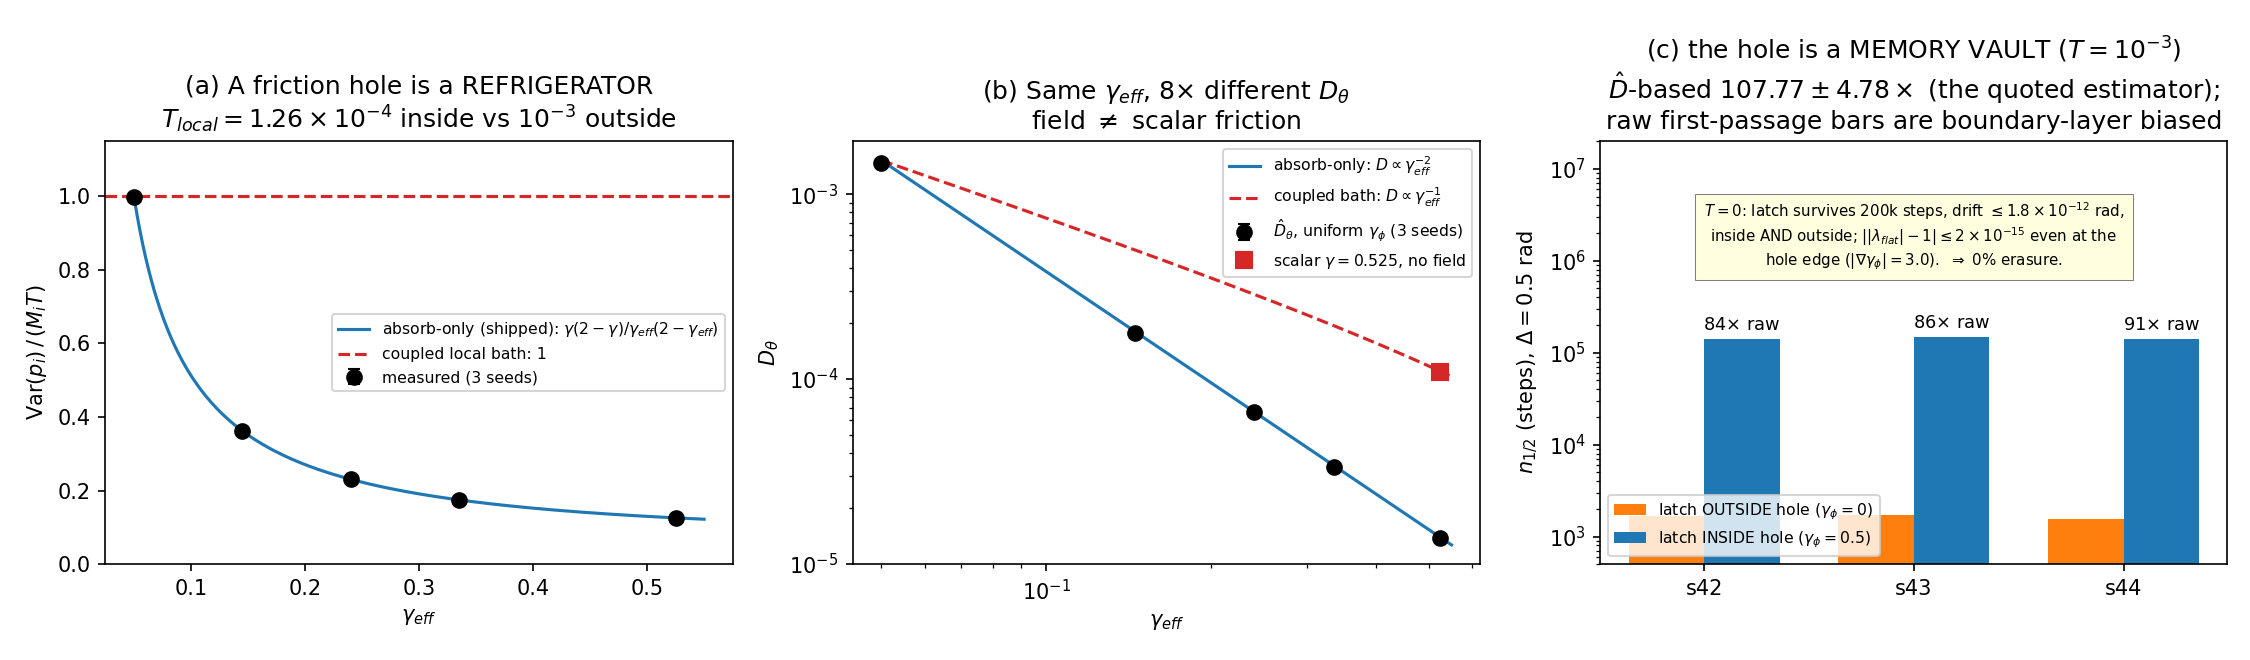
\includegraphics[width=0.70\linewidth]{figs/fig2_vault.png}
\caption{The friction hole as a memory vault. Same effective damping $\gamma_{\rm eff}$, $8\times$ different diffusion: the shipped absorb-only field cools the local bath ($T_{\rm local}=1.26\times10^{-4}$ vs. $10^{-3}$), so a $\gamma_\phi$ hole is a $107.77\pm4.78\times$ vault where a scalar friction of equal $\gamma_{\rm eff}$ gives $13.28\pm0.12\times$; at $T=0$ the hole erases nothing. The quoted vault is the $\hat D_\theta$ estimator, stated on panel (c); the per-seed bars beneath it are raw first-passage ratios ($84$/$86$/$91\times$), which are boundary-layer biased on the outside arm and are not the quoted number (D.3). \emph{(Designed $SO(2)$ + analytic field, 3 seeds, $\Delta=0.5$ rad, laptop-CPU $\Rightarrow$ verification; \texttt{langevin\_noise="fdt"}, Newtonian kinetic mode.)}}
\end{figure}

\textbf{D.7 The vault on an emergent register: two laws transfer, the contrast number does not} \emph{(source: \texttt{v5-vcurve-validation} ME-3. Provenance A.10. Pre-registered. Emergent MLP, 3 seeds $\Rightarrow$ evidence.)}

\emph{Estimator, and why it had to be rebuilt.} On a designed checkpoint the coset is exactly flat, $\mathrm{MSD}_\theta(n)$ grows linearly forever and the fixed-block estimator of B.1 is valid. On an emergent checkpoint the coset is a \textbf{bounded} mode ($\mu^2_{\rm adiab}=2.77\times10^{-2}$--$8.93\times10^{-2}$), so the MSD saturates and that estimator is biased low by up to $55\%$. Two replacements are used and both are reported: $\hat D_{\rm lin}$, the MSD slope over $[n_{\rm lo},n_{\rm hi}]$ with $n_{\rm lo}=4/\gamma_{\rm eff}$ and $n_{\rm hi}$ the largest lag whose local exponent $d\log\mathrm{MSD}/d\log n$ is still $\ge0.90$ (usable only if $n_{\rm hi}\ge2n_{\rm lo}$); and $\hat D_{\rm ou}$ (primary, window-free), the two-parameter fit $\mathrm{MSD}(n)=A(1-e^{-n/\tau})$ over $n\ge n_{\rm lo}$ with $\hat D=A/(2\varepsilon\tau)$, exact for an Ornstein--Uhlenbeck coordinate and degenerating to the linear estimator as $\tau\to\infty$. Both were cross-validated against the banked designed numbers before being used on emergent (A.10).

\textbf{(a) The refrigerator law transfers exactly.} $\mathrm{Var}(p_i)/(M_iT)$, 2048 walkers $\times$ 40 samples, 3 seeds:

\begin{table}[t]\centering\small
\begin{tabular}{p{0.115\linewidth}p{0.115\linewidth}p{0.115\linewidth}p{0.115\linewidth}p{0.115\linewidth}p{0.115\linewidth}p{0.115\linewidth}p{0.115\linewidth}}
\toprule
$T$ & $\gamma_\phi$ & $\gamma_{\rm eff}$ & absorb-only prediction & coupled-bath prediction & measured & obs/absorb & obs/coupled \\
\midrule
$4\times10^{-3}$ & $0.0$ & $0.050$ & $1.00000$ & $1.0$ & $0.99815\pm0.00257$ & $0.9981$ & $0.9981$ \\
$4\times10^{-3}$ & $0.1$ & $0.145$ & $0.36249$ & $1.0$ & $0.36326\pm0.00067$ & $1.0021$ & $0.3633$ \\
$4\times10^{-3}$ & $0.2$ & $0.240$ & $0.23082$ & $1.0$ & $0.23062\pm0.00080$ & $0.9991$ & $0.2306$ \\
$4\times10^{-3}$ & $0.3$ & $0.335$ & $0.17480$ & $1.0$ & $0.17473\pm0.00046$ & $0.9996$ & $0.1747$ \\
$4\times10^{-3}$ & $0.5$ & $0.525$ & $0.12591$ & $1.0$ & $0.12592\pm0.00055$ & $1.0001$ & $0.1259$ \\
$8\times10^{-3}$ & $0.5$ & $0.525$ & $0.12591$ & $1.0$ & $0.12548\pm0.00032$ & $0.9966$ & $0.1255$ \\
\bottomrule
\end{tabular}
\end{table}

Over all 24 field cells ($\gamma_\phi>0$, both temperatures, 3 seeds) obs/absorb $=0.9998\pm0.0019$; at $\gamma_\phi=0.5$, $T_{\rm local}/T=0.12570$, a $7.955\times$ refrigerator against $7.942$ predicted. The coupled-bath hypothesis, which predicts $1.0$ at every $\gamma_\phi$, is measured at $0.2235$ and is \textbf{rejected on an emergent checkpoint as decisively as on a designed one}.

\textbf{(b) The $\hat D_\theta\propto\gamma_{\rm eff}^{-2}$ law transfers.} Restricted to cells whose register is bounded ($\sigma^{\rm ou}_\theta<2\sigma^{\rm Boltzmann}_\theta$; the criterion and its per-cell values travel with the data): $\hat D_{\rm ou}/D_{\rm absorb}=1.0480$ ($\gamma_\phi=0$, 1 cell), $1.1026\pm0.0799$ ($0.1$, 4), $1.0158\pm0.0519$ ($0.2$, 5), $1.0552\pm0.0496$ ($0.3$, 5), $1.0418\pm0.0519$ ($0.5$, 6); against the coupled-bath prediction the same cells give $0.1312\pm0.0065$ at $\gamma_\phi=0.5$. \textbf{Law-referenced vault $D_{\rm absorb}(\gamma_\phi=0)/\hat D(\gamma_\phi=0.5)=106.1\pm5.0\times$} (6 cells; prediction $110.25\times$; banked designed $107.77\pm4.78\times$). A measured/measured ratio over the same cells reads $297.8\pm196.8\times$ (median $234.4\times$); it is recorded here and is never the vault number, because 5 of the 6 $\gamma_\phi=0$ cells fail the bounded test ($\sigma^{\rm ou}_\theta=0.42$--$885$ rad against a Boltzmann $0.24$--$0.65$), so the outside arm is not a register at these temperatures. Every $\gamma_\phi\ge0.2$ cell passes it.

\textbf{(c) The field/scalar contrast number is designed-only, and the failure mode is the control.} The scalar-$\gamma$ laundering control ($\gamma=\gamma_{\rm eff}=0.525$, no field) travels beside every field number. Half of it transfers and half does not. \emph{Transfers:} a scalar $\gamma$ does not cool --- $\mathrm{Var}(p)/(M T)=0.99288\pm0.02354$ at $\gamma=0.525$, where both hypotheses predict $1.0$, against $0.126$ for the field at the same $\gamma_{\rm eff}$; so the mechanism sentence ("a friction field is not locally stronger friction; it is locally stronger friction \textbf{plus} a local refrigerator") stands on emergent. \emph{Does not transfer:} the contrast measures $23.39\pm10.06$ on emergent (per-cell $9.14/25.75/26.96/21.70/41.31/15.48$) against a pre-registered band $[6.5,9.5]$ and a falsifier at $>14$ --- \textbf{the falsifier fired.} The named cause is the control arm, not the field: at $\gamma=0.525$ with no cooling the emergent coset is still anharmonically delocalised, $\hat D_{\rm ou}/D_{\rm flat}=1.1768/3.7319/3.3782/2.7999/5.2284/2.0506$, while the field arm sits on the absorb law at $1.02$--$1.15$. The identical estimator on designed returns $8.03\pm0.80$ (banked $8.11\pm0.37$). \textbf{The contrast direction transfers; the contrast number is a designed quantity and is quoted as one.}

\textbf{(d) New on emergent, with no designed analogue: the hole confines the register.} $T=4\times10^{-3}$, 1024 walkers, burn $20\,000$--$80\,000$ steps ($\ge15$ relaxation times), spread by interquartile range (insensitive to hoppers); "hop" $=|\theta|>1$ rad:

\begin{table}[t]\centering\small
\begin{tabular}{p{0.131\linewidth}p{0.131\linewidth}p{0.131\linewidth}p{0.131\linewidth}p{0.131\linewidth}p{0.131\linewidth}p{0.131\linewidth}}
\toprule
seed & arm & $\gamma_{\rm eff}$ & $\sigma_\theta$ (IQR) & hop fraction & Boltzmann at $T_{\rm local}$ & obs/pred \\
\midrule
42 & no hole, $\gamma=0.05$ & $0.050$ & $0.40795$ & $5.50\%$ & $0.24073$ & $1.6946$ \\
42 & scalar $0.525$ (control) & $0.525$ & $0.20034$ & $0.73\%$ & $0.24073$ & $0.8322$ \\
42 & \textbf{$\gamma_\phi$ hole} & $0.525$ & $0.06442$ & \textbf{$0.0000$} & $0.08542$ & $0.7542$ \\
43 & no hole & $0.050$ & $1.17601$ & $42.97\%$ & $0.46059$ & $2.5533$ \\
43 & scalar $0.525$ & $0.525$ & $0.35335$ & $10.20\%$ & $0.46059$ & $0.7672$ \\
43 & \textbf{$\gamma_\phi$ hole} & $0.525$ & $0.08628$ & \textbf{$0.0000$} & $0.16343$ & $0.5279$ \\
44 & no hole & $0.050$ & $0.36922$ & $2.36\%$ & $0.24034$ & $1.5363$ \\
44 & scalar $0.525$ & $0.525$ & $0.21574$ & $0.26\%$ & $0.24034$ & $0.8977$ \\
44 & \textbf{$\gamma_\phi$ hole} & $0.525$ & $0.07279$ & \textbf{$0.0000$} & $0.08528$ & $0.8535$ \\
\bottomrule
\end{tabular}
\end{table}

With the hole on, the hop fraction is $0.0000$ on 3/3 seeds and the spread sits at $0.53$--$0.85$ of its Boltzmann value at the local temperature; at the same $\gamma_{\rm eff}$ with no cooling it is $0.26$--$10.2\%$. \textbf{The refrigerator converts a hopping rotor into a bounded register, and the laundering control shows that friction alone does not.} \textbf{The pre-registered stationary-spread comparison is void on these checkpoints and no in/out spread ratio may be quoted from them:} its own control, which must return exactly $1.000$ because an equilibrium spread cannot depend on $\gamma$, returns $0.4586\pm0.1181$, so the outside arm has not reached a stationary distribution at $T=4\times10^{-3}$ --- the ratio was registered against a reference that does not exist there.

\textbf{(e) The direct first-passage vault, and the confound it exposed.} \textbf{On an emergent checkpoint the potential has no rotational symmetry, so the banked design's "outside" arm at $\theta=\pi$ is not a vacuum:} $|\nabla V|=0.0420/0.1049/0.0414$ at $\theta=\pi$ against $0.0000$ at $\theta=0$, with $V(\pi)-V(0)=+0.03163/+0.06003/+0.04315$ and $\mu^2_{\rm adiab}$ differing by up to $2.15\times$ between the two sites. \textbf{Any emergent first-passage number quoted against a $\theta=\pi$ baseline is confounded}, and a same-site ($\theta=0$, no field) baseline is required. First passage to $|\Delta\theta|\ge0.5$ rad at $T=4\times10^{-3}$, $\gamma=0.05$, 256 walkers, localized hole of radius $1.0$ centred on \texttt{Ring(0)} (field verified at $0.500000$ at the hole centre and at the exit edge, $0.000000$ at $\theta=\pi$):

\begin{table}[t]\centering\small
\begin{tabular}{p{0.131\linewidth}p{0.131\linewidth}p{0.131\linewidth}p{0.131\linewidth}p{0.131\linewidth}p{0.131\linewidth}p{0.131\linewidth}}
\toprule
seed & $\theta=\pi$, no hole & $\theta=0$, no hole (same-site control) & $\theta=0$, hole & censored & same-site vault & scalar control ($\gamma=0.525$, $\theta=\pi$) \\
\midrule
42 & $1245$ $[930,2203]$ & $725$ $[590,880]$ & $>10^6$ & $86.7\%$ & $>1379\times$ & $3995\to3.21\times$ \\
43 & $295$ $[230,365]$ & $255$ $[225,295]$ & $9050$ $[5950,12556]$ & $0.0\%$ & $35.5\times$ & $2370\to8.03\times$ \\
44 & $15585$ $[9315,21200]$ & $775$ $[680,950]$ & $>10^6$ & $93.4\%$ & $>1290\times$ & $4280\to0.27\times$ \\
\bottomrule
\end{tabular}
\end{table}

The pre-registered $>300\times$ holds on 2/3 seeds as censoring-limited \textbf{lower bounds}, not measurements ($86.7\%$ and $93.4\%$ censored at a $10^6$-step cap; closing them needs $\approx10^7$ steps per walker). The falsifier fires on seed 43 at $35.5\times$; that seed is the one already flagged as geometrically atypical --- softest $\mu^2$, shallowest barrier ($6.8\times10^{-3}$) --- and at $T=4\times10^{-3}$ its coset sits at $\sigma_\theta/\Delta=0.92$ outside and $0.33$ inside, never leaving the diffusive regime, so it gets no Kramers enhancement. The $\theta=\pi$ column is printed only to show the confound: seed 44's $\theta=\pi$ number is $20\times$ its own $\theta=0$ number, and its scalar control reads $0.27\times$ --- raising $\gamma$ by $10.5\times$ apparently \emph{speeding} escape, which is impossible for a stationary register and is the signature of launching walkers on a slope.

\textbf{(f) Scope and confounds carried by all of D.7.} Three emergent model seeds, single PRNG stream per cell, so every spread quoted is across model seeds and not across noise realizations. Both temperatures are above $T^\star\approx3\times10^{-3}$ and the trustworthy-cell restriction of the designed study is $T\le3\times10^{-3}$, so every measurement here is squeezed between $T^\star$ and the onset of delocalisation; only cells passing the printed bounded test support a law claim. The localized hole is a ball of radius $1.0$ in the full 4-D space, so radial or spectator excursions of order $1.0$ ($\approx4.5\sigma_r$ at $T=4\times10^{-3}$) leave it --- a plausible contributor to seed 43's low vault, not separately measured. No temperature field was built.

\begin{figure}[t]
\centering
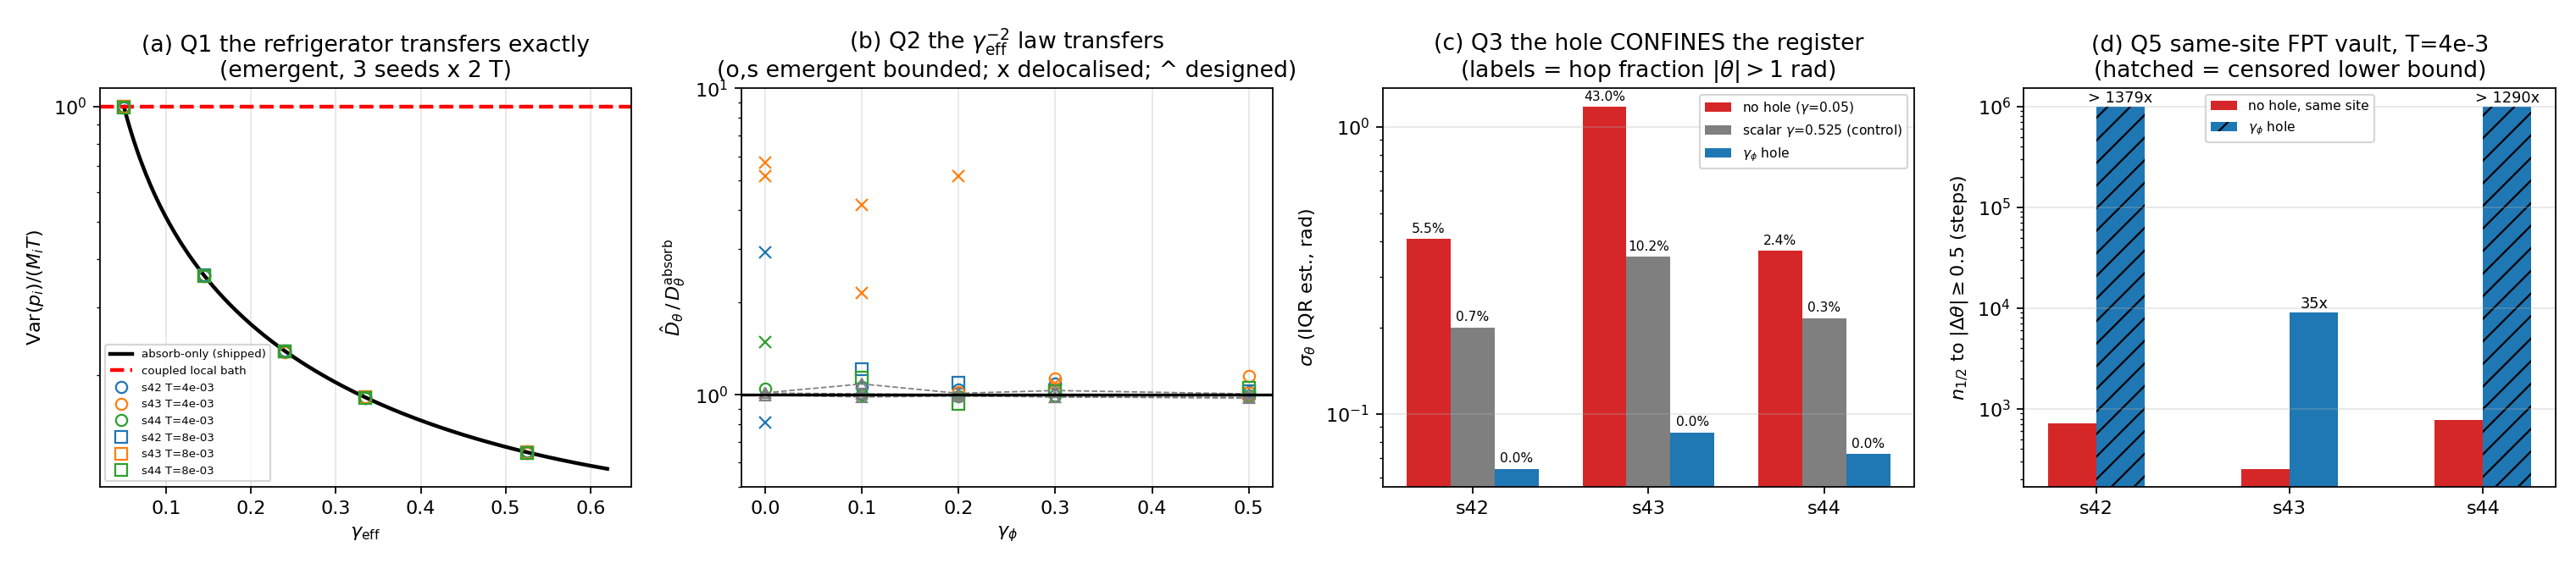
\includegraphics[width=0.70\linewidth]{figs/figD_emergent_vault.png}
\caption{\textbf{Figure D.2.} The vault on an emergent register. Panels are labelled by the pre-registered prediction each tests. (a) The refrigerator law: $\mathrm{Var}(p_i)/(M_iT)$ against $\gamma_{\rm eff}$ for 3 seeds $\times$ 2 temperatures, on the absorb-only curve, with the coupled-bath prediction (dashed) rejected. (b) The $\gamma_{\rm eff}^{-2}$ diffusion law: $\hat D_\theta/D^{\rm absorb}_\theta$ per cell, bounded cells as circles/squares, delocalised cells as crosses, the designed cross-check overlaid. (c) Confinement: the stationary spread and the hop fraction $|\theta|>1$ rad for no hole, the scalar control and the hole. (d) Same-site first passage, hatched bars being censored lower bounds. \emph{(Emergent MLP, 3 seeds, $T\in\{4,8\}\times10^{-3}$, $\Delta=0.5$ rad, \texttt{langevin\_noise="fdt"}, Newtonian kinetic mode $\Rightarrow$ evidence; provenance A.10.)}}
\end{figure}

\section{The deletion estate in full}

\emph{(Sources: \texttt{order-independent-placement} (E.1--E.2), \texttt{placement-landing} (E.3), \texttt{deletion-waitlist-stiffness} (E.4, E.6), \texttt{mia-decay-measurement} (E.5). Provenance A.5--A.8. Designed store, no learning anywhere $\Rightarrow$ verification of the mechanism's exactness.)}

\textbf{E.1 The placement rule.} Each item is a record $r=(\text{key }\kappa,\text{ payload }a,\text{ leak }\lambda,\text{ permanent},\text{ born})$. The store geometry $G$ fixes an address disk of radius $R$ and a hex lattice $\Lambda$ of cells with spacing $d_{\rm safe}$, anchored at the origin, kept iff $|c|\le R$. Three deterministic per-key functions (splitmix64-based): a hash point $g(\kappa)$ uniform in the disk, a 64-bit priority $\mathrm{prio}(\kappa)$ (strict total order, tie-broken by key), and a probe order $\pi(\kappa)$ = all cells of $\Lambda$ sorted by $(|c-g(\kappa)|,\text{cell index})$. \textbf{Canonical placement}: process the live keys in descending priority; each key takes the first cell of its own probe order not already taken by a higher-priority key. The store is then the atoms at those cells with their payloads and current amplitudes, slots packed in priority order. There is no "conflict event" to resolve, because the configuration is defined globally and maintained incrementally by bounded fix-ups; the 400-candidate stochastic search of the previous allocator is replaced by a deterministic assignment that is simultaneously the admission gate (spacing is a lattice invariant) and the placement rule.

\textbf{E.2 The theorems --- and whose they are.} Under distinct keys, fixed geometry and deterministic float ops: \textbf{(T1)} the store is a \textbf{set function} of the live records (strong induction over keys in decreasing priority --- no arrival order appears in the definition); \textbf{(T2)} \textbf{deletion equals set-minus bit-exactly} (via a suffix-stability lemma), realised by removal plus a fix-up cascade; \textbf{(T3)} the spacing certificate holds by construction --- the admission test is absorbed into the geometry (neighbour gradient factor $e^{-4.4^2/2}=6.3\times10^{-5}$); \textbf{(T4)} \textbf{decay and permanence commute with deletion} ($\text{tick}\circ\text{delete}_i=\text{delete}_i\circ\text{tick}$ on survivors). \textbf{Attribution, stated wherever these theorems appear:} \emph{"our placement rule is the \textbf{Blelloch--Golovin (FOCS'07)} stable-matching table with a global priority order and a metric-induced probe order; Theorems 1--2 follow from theirs, and the fix-up cascade is theirs. What is new is the composition: a lattice \textbf{packing certificate}, \textbf{continuously decaying content with a proven delete/decay commutation}, a canonical \textbf{energy function} read by a dynamical relaxation, and --- against a literature that proves strong history independence can cost an exponential slowdown (Buchbinder--Petrank) --- a \textbf{negative} price."} Two clarifications travel with that block. \emph{Naming:} Blelloch \& Golovin do not use the phrase "fix-up cascade"; it is our name for the \texttt{NEXT}-chain delete-time repair of their Figure 1, and the algorithm is theirs either way. \emph{Scope of the exponential separation:} Buchbinder \& Petrank's gap is between the \textbf{weak and strong} history-independence notions, for comparison-based structures such as heaps and queues; our comparison is against a history-\emph{dependent} stochastic relocation rule, so the two statements are adjacent rather than identical.

The extended lineage we use in Related Work is: uniquely represented (canonical) data structures date to Snyder (FOCS'77), further studied by Sundar \& Tarjan and by Andersson \& Ottmann; \emph{obliviousness} --- a distributional condition on the memory representation, which explicitly does not require canonical representation --- is Micciancio's (STOC'97); the weak and strong history-independence notions used here are Naor \& Teague's (STOC'01), characterised by Hartline et al. (Algorithmica 2005) --- cited for the definitional equivalence only, never inside a proof, since their theorem requires a \emph{reversible} structure and our amplitude layer is not; the open-addressed realisation is Blelloch \& Golovin's (FOCS'07); and Blelloch, Golovin \& Vassilevska (SWAT 2008) had already taken unique representation into computational geometry. Accordingly we claim no priority over order-independent placement and no novelty for the displacement rule or its delete-time repair --- both are Blelloch \& Golovin's --- and every exactness statement in this paper is qualified by its scope (store level; below capacity or under set-function eviction).

\textbf{E.3 Exactness, measured at 0 tolerance, and the shipped landing.} Reference implementation: 24 exhaustive orders ($n=4$) + 200 random orders at $n\in\{8,16,40,64\}$ + 100 write/delete interleavings + mid-decay deletes --- \textbf{all bit-identical} (\texttt{tobytes()} equality), minimum spacing exactly $1.540000$; on the shipped store PyTree, \texttt{centers/payloads/amps/active} byte-equal and $V(q)$ byte-equal on 64 random queries (max $|\Delta V|=0.0$) $\Rightarrow$ zero production-code change to the store class. In shipped code the rule is a placement module (286 lines, pure numpy) plus a \texttt{Controller(placement="canonical", lattice\_radius=R)} path, a \texttt{Controller.delete(item\_id)} verb implementing T2 with the fix-up cascade, an array scrub on eviction (the previous build cleared only the active mask and amplitudes, leaving centres and payloads verbatim --- invisible to $V$, so no measured result moved, but \emph{"the item is gone"} was false at the data-structure level), and a hard construction error for \texttt{canonical} + recency eviction. \textbf{Acceptance test (the same adversary harness that measured the leak):} all six statistics $0.5000\pm0.0000$, byte-equal $3\,072/3\,072$ worlds.

\textbf{The packing price, measured under the shipped read.} At $K=64$ the canonical rule admits $61/64$ offered keys deterministically ($\sigma=0$), with per-admitted success $1.0000$ and per-offered $0.9531$; inflating the sizing by $\times1.05$ gives $64/64$ and per-offered $1.0000$. The stochastic refuse-and-relocate allocator it replaces admits $43/64$ on the same seeds, per-offered $0.6719$. That measurement is the content of "the packing price of exactness is negative": canonical placement is not paid for in capacity here, it buys capacity. Delete-time churn is $2.836$ moves per delete at the full $61$-cell load.

\textbf{E.4 The load sweep, and the overflow scope clause.} With the waitlist (refused records kept in a side structure, admission re-run by priority on any delete), exactness holds at \textbf{every load measured, 2 $\to$ 12 offers into a 7-cell lattice = $0.29\times$--$1.71\times$ lattice capacity}: AUC $0.5000\pm0.0000$ on all six statistics, byte-equal $1.0000$ (3 072 worlds per cell, 3 seeds $\times$ 8 targets), under \texttt{budget >= n\_cells}, \texttt{leak = 0}, \texttt{evict\_policy="depth"}. \textbf{Without} the waitlist, at overflow, exactness fails and the scope clause is mandatory: with 7 cells and 8 offers a background item refused in the IN world does not counterfactually return, giving $\mathrm{AUC}(n_{\rm live})=1.00000\pm0.0000$ and white-box address-depth $\mathrm{AUC}=0.91409\pm0.0813$ (TPR $0.989$ @ FPR $1\%$), byte-equal fraction $0.0000$. A pre-registration that failed informatively: $\mathrm{AUC}(z_{\rm hole})\ge0.85$ was registered at overflow and measured $0.576$ --- the fix-up cascade \emph{fills} the freed cell with a re-placed survivor, so the hole moves away from the deleted centre; the overflow leak is real but lives in $n_{\rm live}$ and the address-depth statistic. One previously published overflow cell was a \textbf{harness artefact} (it deleted a stale slot whose priority is lowest, so the delete fell through to eviction on a background row); the genuine overflow failure is the high-priority-target cell, reproduced to 4 dp. Recency-based eviction is intrinsically history-dependent and permanently excluded; the overflow numbers are never the deletion claim.

\textbf{E.5 The leakage curve, in full.} Designed store, shipped two-phase read, no learning anywhere; 8 targets $\times$ 3 seeds = 24 per-example values, 128 paired IN/OUT worlds per target, 18 amplitude levels. \textbf{(i)} Against an \emph{exact} adversary, decay buys nothing: white-box per-example AUC $=1.000$ at all 18 amplitude levels down to the floor; what decays is the effect size --- the depth gap is $0.3935\cdot A$ to four decimal places at every level (the pre-registered closed form $1-e^{-1/2}$) and $d'$ falls $1\,560\to79.6$, exactly linear in $A$. The pre-registered falsifier fired on the AUC metric, as registered. \textbf{(ii)} \emph{The store stops answering before it stops leaking}: at the last amplitude before self-eviction ($A=0.051$, $\tau=2.976$) retention is $0.832$ while query-MIA is AUC $0.983$ (TPR $0.858$ @ FPR $1\%$) and white-box $1.000$; the curves never cross, the gap opening from $0.000$ ($\tau\le1.2$) to $+0.151$ at the floor. \textbf{(iii)} Against a \emph{resolution-limited} adversary the grading is real and the pre-registered law survives: $A_{75}=2.57\sigma_{\rm obs}$ measured $0.0780/0.2627/0.7537$ at $\sigma_{\rm obs}=0.03/0.1/0.3$ against predicted $0.0771/0.2570/0.7710$ ($+1.2\%,+2.2\%,-2.2\%$), the whole $\mathrm{AUC}(A)$ curve lying on the registered $\Phi(0.3935A/1.5\sigma)$ --- but $\sigma_{\rm obs}$ is \emph{our modelling choice}, so its defensible use is mechanistic ("the leak signal is $0.3935\cdot A$"), never protective. \textbf{(iv)} Mechanism: the background contributes $e^{-4.4^2/2}=6.3\times10^{-5}$ at the target centre while the target still contributes $0.3935A\ge0.0197$ at the floor, so separation shrinks but never reaches the (zero) noise floor of a \emph{paired} adversary. Against a natural-history OUT adversary the white-box curve \textbf{is} graded ($1.000\to0.791$). \textbf{(v)} \emph{State the $|c|$ distribution with any retention number.} Every retention magnitude in this paper is for the controller-placed disk of A.7 (proposal disk $R=2.2869$, packing bound $8.00$); on a max-radius ring, where every site sits at the same maximal $|c|$, the same store gives retention $0.500$ at $A=0.06$ where this placement gives $0.886$. The one differentiator needing no adversary caveat is retrieval geometry: $R_{50}$ contracts $1.146/1.083/0.979/0.874/0.752$ as $A:1\to0.5\to0.2\to0.1\to0.06$ --- a $1.52\times$ contraction matching the pre-registered saddle prediction at all five points ($\pm0.20$) --- while a TTL vector-store's lookup radius is a constant hard step at $0.75$--$0.77$, independent of age. Quote-the-curve: every load-dependent statistic here is quoted at its load ($7/8$ of the packing bound is the most favourable case for a hole statistic; an occupancy sweep is owed before any such number is generalized). We make no claim that decay reduces distinguishability per se, and no $(\varepsilon,\delta)$ claim of any kind.

\textbf{(vi) The tighter laundering control, and it fires.} The pre-registered control for "physical amplitude beats a bookkeeping flag" is a CLU whose amplitude is replaced by a boolean TTL flag inside the \emph{same} store: identical store, controller, adversary, worlds and queries, with \texttt{amp $\equiv$ 1} until the same expiry tick and then \texttt{evict}. Measured at $A=0.06$:

\begin{table}[t]\centering\small
\begin{tabular}{p{0.23\linewidth}p{0.23\linewidth}p{0.23\linewidth}p{0.23\linewidth}}
\toprule
adversary & CLU physical decay & CLU with a TTL flag & separation \\
\midrule
white-box, exact & $1.000$ & $1.000$ & $0.000$ \\
query-MIA, exact & $0.983$ & $1.000$ & $0.017$ \\
query-MIA, $\sigma_{\rm obs}=0.1$ & $0.559$ & $0.996$ & $0.437$ \\
\bottomrule
\end{tabular}
\end{table}

Against an exact adversary a boolean flag and an $e^{-\lambda t}$ amplitude are equally detectable, so at the AUC level there is \textbf{no measurable differentiator} --- the control fires. It fails to fire only against a resolution-limited adversary, and that resolution is our modelling choice. This is why the differentiator we lead with in the main text is (v)'s retrieval geometry, which needs no adversary model: it is the honest survivor of this control, not a preferred metric.

\textbf{E.6 The trilemma and the gated-stiffness channel.} \emph{"With a quadratic payload channel, the $q_2(0)=0$ anti-decoration guard and a fixed read budget, a store cannot have all three of exact value fidelity, amplitude-independent address hold and amplitude-independent read latency --- pick two. The shipped store drops the second, which is why effective lifetime correlates $r=-0.85$ with $a_i^2$; the recommended gated-stiffness channel drops the third."} Both previously proposed repairs are \textbf{refuted and neither is available}: multiplying payloads by amplitudes kills the value criterion at $A=1-\text{tol}/|a_i|$ (measured death amplitudes $0.90/0.80/0.70/0.30$ against the formula's $0.900/0.860/0.767/0.300$ --- exact) and \emph{inverts} the payload dependence; launching the payload coordinate at the address-mapped point breaks the anti-decoration guard --- a trivial substitute then passes $0.672$ of queries with no dynamics at all, amplitude-independently. The gated-stiffness channel ships behind a flag, default off, with $V$ bit-identical when off: $R_{50}$ contracts $1.135\to0.771$ under the gate (baseline $1.146\to0.752$), retention std $0.274\to0.016$ and worst codeword $0.398\to0.972$. The registered payload-independence test was a \emph{correlation} and \textbf{fails as stated} ($|r|$ only $0.846\to0.667$): a correlation is the wrong statistic once the quantity it correlates with stops varying, so we report the effect sizes (retention std, worst codeword) and not the correlation coefficient. At $\gamma_{\rm read}=0$ the gated channel is \textbf{oscillatory}, period $2\pi/\sqrt{\kappa(g_0+A)}$ (measured log-log slope $-0.5264$), not relaxational, so no $\tau\propto1/A$ settling law may be quoted without a nonzero read friction. The graded configuration ($g_0\ll$ \texttt{amp\_floor} plus a longer read as the item fades) is the \textbf{compute-adaptive-read} dial --- and it is \emph{not} the shipped arm.

\textbf{E.7 Citation and vocabulary discipline.} \emph{Certified} removal is introduced by Guo et al. (ICML 2020) in \textbf{\S 2} as $\varepsilon$-certified removal, \textbf{Eq. (1)}, with a relaxed $(\varepsilon,\delta)$ notion stated as an unnumbered display immediately after; neither is a numbered Definition, and we cite it that way; we do not use the word for anything in this paper's mechanism. Cost and capacity formalisms already exist and are adopted rather than re-coined (Ginart et al., NeurIPS 2019, \textbf{Def. A.5}, amortized time; Sekhari et al., NeurIPS 2021, \textbf{Def. 3}, deletion capacity at fixed excess risk), with SISA's (Bourtoule et al. 2021) shards-vs-accuracy curve as the practice precedent and \textbf{the flat-datastore row-delete as the mandatory trivial substitute}. \textbf{No deletion-cost statement is made here}: the shipped canonical synchronisation is a full $O(n)$ rebuild per operation, and the amortized-cost experiment has not been run. Nor do we claim uniqueness --- a table deletes exactly by construction, and a 2026 preprint publishes unlearning-by-design for a memory-augmented transformer, evaluated on the same membership instrument (forget-set MIA AUROC $\to51.4\%$ / $51.2\%$ on CIFAR-10 / DermaMNIST at a $10\%$ forget set). It is not exact: its average gap to the retrained oracle, across four metrics, is $0.56\pm0.21$ (Laguna et al., 2026, arXiv:2603.15033).

\section{The three-state lifecycle in full (mechanics)}

\emph{(Source: \texttt{c2w10-lifecycle-mechanics}. Provenance A.9. Toy synthetic build, 3 seeds, \texttt{addr\_dim = 12}, 64 live wells $\Rightarrow$ a \textbf{mechanics instrument, never a claim venue}. No value/benchmark cell accompanies this build; that surface is a \textbf{declared not-run}, not a null.)}

\textbf{F.0 The lifecycle statement, in full (banked from the main text at the 4 pp cut).} \emph{(Toy synthetic build, 3 seeds, \texttt{addr\_dim = 12}, 64 live wells; A.9, leg table below.)} These compose into a lifecycle we ship and exercise: \textbf{PROTECTED $\rightleftarrows$ ACTIVE $\to$ TRASH, 7/7 legs, kill-conditions committed BEFORE the verbs, every designed negative shipping with the named mutation that makes it fail; L4 labelled UNEXERCISED (0 refusals on the stream).} Two riders travel with it: \textbf{demotion is re-exposure to designed decay, never the trash region}, and \textbf{the trash criterion is keyed on \texttt{read\_hits}, never on depth}. \textbf{Scope:} a mechanics demonstration on a toy synthetic build --- an instrument, never a claim venue; no value or benchmark measurement accompanies it, and that surface is a \textbf{declared not-run}, not a null.

The build order was \textbf{kill-conditions first}: the designed negatives were committed against an unimplemented module and observed RED (32 failed, 1 passed --- the single green test inspects the criterion's \emph{signature} for a depth argument, which the stub also lacked), and only then was the implementation committed. \texttt{lifecycle\_mechanics\_done} is computed in code as the AND over the seven legs, each of which is a test exit status, not a judgement.

\begin{table}[t]\centering\small
\begin{tabular}{p{0.23\linewidth}p{0.23\linewidth}p{0.23\linewidth}p{0.23\linewidth}}
\toprule
leg & landed & designed negative(s) & shown able to FAIL by \\
\midrule
\textbf{L1 promotion} &  & a single usage burst reaching the high threshold does \textbf{not} promote (dwell $2<3$); a well below the low threshold never promotes & setting dwell $:=$ window $\Rightarrow$ the burst \textbf{does} promote; high threshold $:=0$ $\Rightarrow$ a never-read well promotes \\
\textbf{L2 demotion} &  & a planted early-popular-then-abandoned well \textbf{demotes within \texttt{d\_demote}} and is \textbf{not} trashed by the demotion; the demoted well's depth follows $\exp(-\text{leak}\cdot\Delta t)$ again & disabling demotion $\Rightarrow$ it stays PROTECTED forever \\
\textbf{L3 trash} &  & (a) useful in stream 1 only $\Rightarrow$ trashed at $k$; (b) useful in \textbf{every} stream $\Rightarrow$ \textbf{never} trashed; (c) censoring guard: a well admitted in the last stream is \textbf{never} trashed & (b) discriminating input flipped (hits zeroed $\Rightarrow$ trashed); (c) guard off $\Rightarrow$ the young well \textbf{is} trashed; (a) criterion switched to since-first-seen $\Rightarrow$ does \textbf{not} fire \\
\textbf{L4 protected fraction} &  & forcing every item's usage high \textbf{trips saturation and REFUSES}, never silently protects everything & cap $:=1.0$ $\Rightarrow$ everything protects and nothing trips \\
\textbf{L5 refresh guard} &  & with the guard off a planted destructive rewrite \textbf{reduces} the depth --- asserted on replayed depths \textbf{and} on the live store path & the same events with the monotone guard on end at $\min(d_{\rm before}, d_{\rm after}\cdot\text{gain}^2)$ \\
\textbf{L6 netting} &  & netted $\equiv$ raw \textbf{bitwise} at zero leak; netted $>$ raw strictly at positive leak; a well with no writes nets to the analytic decay law & the same function on both branches, plus the float32-floor bound \\
\textbf{L7 off-switch} &  & OFF is \textbf{bit-identical} (leaves and read output) and parameter-count-identical; the trash region is attached only when the verb is on & --- \\
\bottomrule
\end{tabular}
\end{table}

\textbf{F.1 L4 is UNEXERCISED, and that is reported, not hidden.} The protected cap is $\lfloor 0.25\times64\rfloor=16$ wells and the measured protected population never approached it, so the saturation path recorded \textbf{0 refusals on the stream}. Per our own registered rule this is reported as \textbf{UNEXERCISED --- not working and not broken}; the verb is green on the planted population (the negative \emph{and} its can-fail twin), what is absent is a \emph{stream} population that reaches the bound. \textbf{Why is measurable, not mysterious:} promotion is sticky (dwell $>$ window) and demotion prompt, while usage at this read budget is bursty on a 2-chunk timescale, so promotions are undone nearly as fast as they are made and the protected set never accumulates. If stable protection is wanted, the demotion delay must exceed the usage's burst gap --- a parameter choice, not a defect.

\textbf{F.2 Two mechanics riders that travel with any statement of the lifecycle.} \textbf{Demotion is re-exposure to designed decay --- never the trash region.} \textbf{The trash criterion is keyed on \texttt{read\_hits} --- never on depth} (depth is not feature importance, and that caveat is active).

\textbf{F.3 Reconciliations owned by this build (recorded, not hidden).} Two prior attributions of event counts to the wrong arm were corrected against the raw artifacts; a "zero post-guard violations" claim that had never been in any artifact was recomputed and now has evidence for the first time; one registered leg wording and its designed negative were shown not jointly satisfiable, so both readings ship with the default declared and the difference asserted in tests; a registered bitwise tolerance holds in float64 but not in the shipped float32 amplitudes (floor $\approx5.3\times10^{-8}$), and both are pinned.

\section{Coleman / Mermin--Wagner, and the mandatory \texttt{fdt} + Newtonian scope}

\textbf{Stated honestly.} A continuous symmetry cannot be spontaneously broken in a $0{+}1$-dimensional \emph{thermal} system (Mermin \& Wagner 1966; Coleman 1973), and our latch does not contradict this: \textbf{the infinite half-life is a $T=0$ statement} about the deterministic damped map. At $T>0$ the coset is a \emph{diffusive register} ($D_\theta=\varepsilon T(2-\gamma)/(2F^2\gamma)$) with a finite, computable lifetime, not long-range order.

\textbf{Mandatory flag, travelling with every $T>0$ number in this paper.} All $T>0$ results require \texttt{langevin\_noise="fdt"} --- the fluctuation--dissipation-consistent noise scale $\sigma^\star_i=\sqrt{M_iT\gamma(2-\gamma)}$ --- \textbf{and} a Newtonian kinetic mode. The reference implementation's default is \texttt{legacy}, under which $T$ is not in energy units and \textbf{none} of these laws hold. In the relativistic kinetic mode the coded damping substep is an additive Gaussian momentum kick of fixed covariance, so the chain's invariant momentum marginal is necessarily Gaussian-smoothed; a relativistic (Maxwell--J\"uttner) Gibbs marginal is not of that form, so \textbf{no} noise scale gives the coded relativistic Langevin a Gibbs invariant at all. The failure is in the \emph{sampler}, not the thermodynamics --- the configurational equilibrium $\pi_q\propto e^{-V_\theta/T}$ is relativity-insensitive. Every checkpoint here uses a Newtonian kinetic mode, so $\sigma^\star$ is exact for every run.

\section{Erosion as symmetry restoration: instance, demarcation, frequency-horizon law, anchor cure}

\emph{(Source: \texttt{sleep-erosion-study}; the novelty search is described at the end of this appendix. Evidence-grade: training dynamics on learned potentials. \textbf{Designed-vacuum scope}; see the rider at the end.)}

At the reference configuration's default 1000 epochs, wake--sleep contrastive-divergence training \textbf{inverts} a designed $SO(2)$ vacuum in 8/8 runs: ring depth $+0.079\to-0.126$, order parameter $r^*:1.0\to0$ (the data ring becomes a local maximum). This is a \textbf{symmetry-restoration (condensate-melting)} event in the classical, tree-level sense --- the minimiser becomes $G$-invariant --- not a thermodynamic phase transition. Four claims, with their attribution held exactly as the source study framed them:

\begin{itemize}
\item \textbf{(a) Inversion of a designed degenerate vacuum} --- \emph{cite the substrate.} That short-run contrastive divergence distorts or diverges an energy landscape is classical (Fischer \& Igel 2010, 2011; Nijkamp et al. 2020). Ours is a sharp, quantified instance on a symplectic, Hamiltonian energy-based primitive. \textbf{We do not claim to have discovered that CD is biased.} The nearest RBM symmetry-breaking result is not a precedent for this claim: it attributes the breaking of an \emph{initialization} symmetry of the weight spectrum to hierarchical feature learning, with CD and PCD appearing only as sampling implementations (Toledo-Mar\'in et al. 2025).
\item \textbf{(b) Degeneracy-specificity demarcation} --- \emph{novel to our knowledge, single-sourced.} Erosion strikes flat directions and \emph{spares} non-degenerate vacua: a non-degenerate sine vacuum is immune (wake+sleep $\approx$ wake-only), because the wake trajectory-MSE objective pins $V$'s value at every data point except along a flat coset it cannot see.
\item \textbf{(c) Frequency-horizon law} --- \emph{novel to our knowledge, single-sourced, practitioner-relevant.} The erosion horizon is set by sleep-update \emph{frequency} racing the wake-clamp schedule, \textbf{independent of chain length}: inversion at epoch $\approx116/442/959$ for sleep frequency $1/5/20$; the number of sleep sub-steps (50 vs 500) is irrelevant to $\pm1$ epoch; persistent-CD vs CD shifts it $\le9$ epochs. \textbf{Scope clause, which travels with (c).} The nearest documented neighbour concerns \emph{chain length}: in RBM/EBM learning the number of sampling steps $k$ relative to the model's mixing time defines equilibrium versus out-of-equilibrium learning regimes, and it does change what is learned (Decelle, Furtlehner \& Seoane 2021; Agoritsas et al. 2023). Our sweep varies chain length only over \texttt{sleep\_steps} $\in\{50,500\}$ at otherwise fixed sampler settings and does not resolve where either sits relative to this model's mixing time, so the finding is \emph{frequency-decisive across the two chain lengths we run}, and is \textbf{not} a claim that chain length is irrelevant to contrastive-divergence learning in general.
\item \textbf{(d) Value-anchor cure} --- \emph{cite the adjacent precedent.} A $V(\text{data})$ energy anchor holds the condensate up ($\lambda=10$: ring depth flat $+0.068$--$+0.072$ over 1000 epochs, $r^*\approx0.96$) and, because sleep is retained, noise rejection \emph{grows} to $+0.244$, beating wake-only $+0.199$. The nearest precedent is the energy-magnitude regularization of Du \& Mordatch (2019), used there for partition-function stability rather than to preserve a structural prior.
\end{itemize}

\textbf{Framing, preserved from the source study:} \emph{we contribute a sharp, quantified instance + demarcation + cheap cure, not the discovery that CD is biased.} Novelty of (b) and (c) is by absence, and that search has been run --- twice, with different query sets and databases (through Aug 2026): arXiv cs.LG / cs.NE / cond-mat.dis-nn / stat.ML; NeurIPS 2020--2025; ICML/PMLR v119, v139, v202, v235; ICLR/OpenReview; AAAI; and the journals \emph{Neural Computation}, \emph{Machine Learning: Science and Technology}, \emph{Frontiers in Computational Neuroscience}, \emph{Mathematics} and \emph{Nature Communications}. It covered the CD/EBM, continual-EBM, equilibrium-propagation and RBM-symmetry-breaking literatures and found no prior statement of either claim. \textbf{That is absence over the surfaces listed, not proof of none:} paywalled journal archives, forward-citation crawls of the CD-bias literature, non-English work and workshop tracks were not searched. \textbf{Scope rider (blast radius, \S 2.2).} The demarcation is a statement about \emph{designed} degenerate vacua: an explicit tilt immunizes such a vacuum with no anchor at all (erosion $\propto$ flatness) on the designed testbed. It does \textbf{not} license a tilt prescription on a \textbf{learned} store, where the analogous claim is refuted in sign and the soft-mode lifetime is capped by the confinement floor ($\tau_{\max}=\Gamma/2\alpha$).

\section{Horizon: a localized temperature field (specified, not built)}

\emph{(Future work; stated as a prediction, not a result.)}

The budget predicts a complementary "shredder": a learned, position-gated hot region $T_\phi(q)\ge0$ that erases latched coset content locally, where a friction hole provably cannot (\S 2.2, D.5). Inside a hot region the coset obeys $D_\theta(q)=\varepsilon T_{\rm tot}(q)(2-\gamma_{\rm eff})/(2F^2\gamma_{\rm eff})$ with $T_{\rm tot}=T+T_\phi$, so the erasure rate is $\propto T_\phi/(\gamma F^2)$. \textbf{Hard design rule (a consequence of \S 2.2, not a caution):} a $T_\phi$ hot spot must \textbf{not} be co-located with a $\gamma_\phi$ hole --- under the shipped absorb-only path, co-location dilutes erasure by $(\gamma_{\rm eff}/\gamma)^2\approx107\times$, so the friction would preserve exactly the content the heat is meant to destroy. The module (compact gate, two-timescale learning rate, contrastive training, mirroring the shipped friction field) is specified and unbuilt; the "shredder" half of the forgetting story is a prediction.

\section{Negatives ledger (future-work anchors)}

\emph{Every negative below is on the record with its measurement; none is dropped, and each is the anchor of a future-work item.}

\begin{enumerate}
\item \textbf{No continuous coset register emerges} (\S 2.2, C.2). An MLP potential trained on symmetric data yields a mid-spectrum massive mode ($1.7$--$4.9\times$ softer than the stiffest mode), capacity $\approx1$--$1.6$ bits, complete relaxation of any written continuum value. The exact $T=0$ latch is designed-only.
\item \textbf{The raw-exponent artifact} (C.5). Raw $T/\gamma$-exponents do not discriminate designed from emergent; a matched designed control reproduces the same shallow slopes. Only $\ell_\theta/\Delta$-controlled cells and $|\lambda_{\rm coset}|$ discriminate. Standing reporting rule: never an $n_{1/2}$ without $\Delta$ and $\ell_\theta/\Delta$.
\item \textbf{The coupled-bath vault prediction is wrong for the shipped code} (D.1). A pre-registered measurement rejected it by a factor $8.11$; the shipped field is absorb-only and the vault is $(\gamma_{\rm eff}/\gamma)^2 = 107.77\pm4.78\times$ measured, with $13.28\pm0.12\times$ the measured scalar-friction control.
\item \textbf{A friction field is the wrong operator to \emph{forget} a coset} (\S 2.2, Appendix I). At $T>0$ it \emph{lengthens} coset memory; erasing latched coset content needs a temperature (or tilt) field. This is the first-principles explanation of the previously observed failure of a learned friction field to recover fit on a stationary vacuum.
\item \textbf{Our own sign-flip prediction was falsified in one of two observables} (C.6): a register written at the washboard minimum cannot flip back, and both signs coexist on one checkpoint for different observables.
\item \textbf{Amplitude decay does not reduce an exact adversary's per-example distinguishability at any point in an item's life} (E.5): white-box AUC $1.000$ at all 18 amplitude levels; what decays is the effect size. The graded curve exists only relative to a stated adversary resolution, which is our modelling choice.
\item \textbf{At overflow, canonical placement without the waitlist is not exact} (E.4): $\mathrm{AUC}(n_{\rm live})=1.000$, byte-equal fraction $0.0000$. Every deletion sentence carries its scope clause; recency-based eviction is permanently excluded.
\item \textbf{The placement algorithm is not ours} (E.2): Blelloch \& Golovin (FOCS'07) own it outright, and unique representation in a geometric setting is also taken (SWAT 2008). Our claim is the composition only.
\item \textbf{A cost claim we cannot make} (E.7): the shipped canonical synchronisation is an $O(n)$ rebuild per operation, so the amortized-deletion-cost formalism of the unlearning literature cannot be instantiated on our own code until that experiment is run.
\item \textbf{Both proposed repairs of the payload-lifetime coupling are refuted} (E.6), and the registered payload-independence statistic failed as registered --- the effect size passes decisively, the correlation does not. At zero read friction the gated channel is oscillatory, not relaxational.
\item \textbf{The pseudo-Goldstone tilt prescription is refuted in sign on a learned store} (K.3): an explicit tilt monotonically \emph{reduces} the smallest eigenvalue on two independent implementations and every family, because a written site is not a common vacuum of its own atoms. The relation survives only in the single-atom geometry it was specified in.
\item \textbf{A tilt is not a lifetime dial on a learned store} (K.3): the confinement floors the soft eigenvalue at $2\alpha$, capping the lifetime at $\tau_{\max}=\Gamma/2\alpha$; the registered damped-mode floor is confirmed, the $1/\text{tilt}$ branch is unreachable, and lowering $\alpha$ breaks the write.
\item \textbf{L4 of the lifecycle is unexercised} (F.1): 0 refusals on the stream at the measured operating point --- reported as unexercised, not as working and not as broken.
\item \textbf{No task-level payoff is claimed} (\S 4): forgetting here is shown predictable, controllable, removable and schedulable --- not shown to improve a downstream metric. \textbf{External benchmarks won on their own headline metric = ZERO.}
\item \textbf{The field/scalar vault contrast does not transfer to an emergent register} (D.7c). It measures $23.39\pm10.06$ there against $8.03\pm0.80$ from the identical estimator on designed; the pre-registered falsifier fired. The cause is the laundering control itself --- at $\gamma=0.525$ with no cooling the emergent coset is anharmonically delocalised ($\hat D/D_{\rm flat}=1.18$--$5.23$) --- so the contrast \emph{number} is designed-only while its direction transfers.
\item \textbf{The emergent stationary-spread diagnostic is not measurable above $T^\star$} (D.7d). Its own control, which must return $1.000$, returns $0.4586\pm0.1181$: the no-hole arm is a hopping rotor, not a stationary register, so no in/out spread ratio may be quoted on these checkpoints. The confinement statement (hop fraction $\to0.0000$) replaces it.
\item \textbf{A $\theta=\pi$ baseline is invalid for first-passage measurements on an emergent checkpoint} (D.7e). $|\nabla V|=0.042$--$0.105$ there against $0.0000$ at $\theta=0$; one seed's scalar control reads $0.27\times$, i.e. more friction apparently speeding escape. Every emergent first-passage number needs a same-site baseline; the designed arm is protected by $SO(2)$ symmetry but was never checked, and that check is owed.
\item \textbf{Threshold instruments are unusable below $\gamma_{\rm crit}$} (C.3.1). A rollout first-crossing $n_{1/2}$ puts its argmin at the grid edge with a below-slope of $+0.0623\pm0.0120$ where the law says $-1$; a last-crossing definition carries an additive half-period bias. Only the envelope-rate instrument is quotable there.
\item \textbf{Our microscopic explanation of the instrument offset was wrong} (C.3.1). The offset itself is real, constant and quotable, but the pre-registered single-slow-mode projection model fails: the measured amplitude fraction $0.638/0.644/0.327$ does not order like the angular overlaps, and the early-window rate ratio $0.52$--$0.85$ is amplitude-independent, i.e. multi-mode transient rather than anharmonicity.
\item \textbf{The emergent first-passage vault is a bound on 2 of 3 seeds and misses on the third} (D.7e): $>1379\times$ and $>1290\times$ at $86.7\%$/$93.4\%$ censoring, and $35.5\times$ on the geometrically atypical seed. Three seeds cannot say which is typical.
\item \textbf{Class-level scope caveats} (theory note, neutral theorems): a \emph{mean}-spectrum chaos regularizer is degenerate (a max/positive-part statistic is required), and the FDT noise scale is exact only in Newtonian kinetic modes (Appendix G). Neither bears on any number here.
\end{enumerate}

\section{Material banked from the main text (page-limit cuts, kept in full)}

\emph{The short track's 4 pp limit forced compression, never deletion: the full form of every compressed main-text passage is preserved here.}

\textbf{K.1 Nomenclature and measurement discipline, in full.} Two quantities are both called "mass" and run in opposite directions: the \textbf{inertial mass} $M_i$ (the learned diagonal of the kinetic term; larger $M\Rightarrow$ slower dynamics) and the \textbf{spectral mass} $\mu_k$ (normal-mode frequency $\mu_k^2=\lambda_k(M^{-1/2}\nabla^2V_\theta M^{-1/2})$ at a critical point; larger $\mu\Rightarrow$ shorter memory). All retention statements use $\mu$; the constitutive identity $\mu^2=\mathrm{eig}(M^{-1}\nabla^2V_\theta)$ is exact on the trained checkpoints used here (the Hessian-derived spectral mass equals the measured one-step-Jacobian gap to $3.2\times10^{-10}$ across the tilt rows measured). A stored analog value lives on a \textbf{coset direction} --- a near-flat ($\mu\to0$) direction of $V_\theta$; the memory it holds is the coset coordinate, and $F^2=M_{\rm ch}r^{*2}$ is that channel's decay constant (current--coordinate coupling on the vacuum orbit of radius $r^*$). \textbf{Notation collision, stated because it is a real hazard across this literature:} $\varepsilon$ here is the integrator step ($\varepsilon=\mathrm{dt}=0.05$) and never an explicit-symmetry-breaking tilt; where a tilt appears (Appendix H) it is written $\delta$. \textbf{The measurement discipline:} a coset half-life $n_{1/2}$ is meaningful only relative to a read tolerance $\Delta$ (the drift at which the value is declared lost) and the thermal persistence length $\ell_\theta=\varepsilon\sqrt{T/M_{\rm ch}}/(\gamma r^*)$ --- a coset register's physical resolution limit at temperature $T$. The pure-diffusion law holds in the limit $\ell_\theta/\Delta\to0$; outside it, raw $n_{1/2}$ inflates predictably (toy/pure-diffusion $-1=3.099(\ell_\theta/\Delta)-0.0059$). Hence: \textbf{never an $n_{1/2}$ without its $\Delta$ and $\ell_\theta/\Delta$}, and never a designed-vs-learned distinction read off raw exponents (C.5).

\textbf{K.2 Related work, in full.}

\emph{Long-term memory for AI systems.} Agent memories are built as external stores that an LLM writes to, retrieves from and edits: MemGPT pages content between a fast context and a slow store under the model's own control (Packer et al. 2023), Mem0 exposes the update phase as a tool call over ADD, UPDATE, DELETE and NOOP (Chhikara et al. 2025), and Infini-attention keeps a bounded compressive state inside the network instead (Munkhdalai et al. 2024). Two design points in that literature are the ones our claims touch. The first is \emph{decay}: Generative Agents score retrieval by recency, importance and relevance, with recency an exponential decay of factor $0.995$ over sandbox hours (Park et al. 2023); MemoryBank decays a memory-strength score along an Ebbinghaus curve (Zhong et al. 2024); Expire-Span learns a per-memory expiration span for efficiency (Sukhbaatar et al. 2021); and Titans updates a test-time memory as $\mathcal M_t=(1-\alpha_t)\mathcal M_{t-1}+S_t$ with $\alpha_t$ a learned forget gate (Behrouz et al. 2025). Each is a heuristic score or a learned hyperparameter; none states a half-life, a read tolerance, or a temperature, and none prices what is lost. Our $(\mu,\gamma,T)$ budget occupies the same functional slot with those three quantities attached --- a contrast in kind, not a competing system, and we run no benchmark against any of them. The second is \emph{removal}: Zep's temporal knowledge graph invalidates contradicted edges by setting an invalidation timestamp and deliberately preserves the historical record (Rasmussen et al. 2025); Mem0's DELETE removes a row from a discrete store. Byte-identity is the opposite design point, and it is only interesting because tombstoned vectors have been shown to remain physically present and reconstructible from raw index files in graph ANN databases (Chakraborttii et al. 2026). Finally, the evaluation wave that motivates the framing: production memory failures are predominantly forgetting failures rather than recall failures while benchmarks measure recall (Yang 2026), failures to forget outdated memory account for a large share of sampled recommendation errors (Uddin et al. 2026), deleted facts remain recoverable through retained correlated modalities even when the text entry is gone (Wang \& Zhang 2026), and agentic unlearning must handle reactivation of forgotten content from persistent memory (Wang et al. 2026). The last two are why \S 2.3's encoder-excluded scope is stated as a scope and not as a hedge: the store deleting an item is not the system forgetting it.

\emph{Dissipative Goldstone modes.} The physics precedent for \S 2.2 is the theory of Nambu--Goldstone modes in \emph{dissipative} systems: Minami \& Hidaka (2018) show that dissipation turns type-A Goldstone modes from propagating to \textbf{diffusive}, and trace the difference to two types of Noether charge; the follow-up classifies the modes into four types (Hidaka \& Minami 2020). Our coset is exactly this --- the $\gamma$ knob converts a propagating Goldstone into a diffusive register with $D_\theta\propto T/\gamma$, and "spending friction" lengthens rather than shortens its memory. We import the propagating$\to$diffusive picture and add its retention consequence (the sign flip) and the explicit discrete-map diffusion constant.

\emph{Equivariant and continuous-attractor dynamics.} The neutrality of group-orbit directions is classical (Golubitsky, Stewart \& Schaeffer 1988; Krupa 1990) and underlies continuous-attractor memory. \textbf{Mo (2026)} proves that an exactly $G$-equivariant recurrent flow has \textbf{at least} $\dim(G/\mathcal H)$ zero Lyapunov exponents along the orbit and shows a "pseudo-gap" predicts finite lifetime --- the \emph{kinematics} of protection, silent on what sets the gap. Our budget is the \emph{constitutive} complement: the gap is $\mu^2$, its retention is the V-curve of \S 2.1, and its $T>0$ decay is diffusive with a computable $D_\theta$. Crucially we do \textbf{not} claim the continuum coset emerges: \S 2.2 shows a generically-trained unit has only a discrete washboard, so equivariant \emph{design} is the precondition --- consistent with Mo's sufficiency statement. \textbf{Di Bernardo et al. (2025)} link connectivity symmetry to the geometry and stability of fixed-point manifolds in equivariant RNNs; they engineer \emph{which} manifold exists, not its dissipation-priced forgetting timescale. \textbf{Iqbal, Keller, Song, Miyato \& Welling (2026)} use spontaneous symmetry breaking with gapless Goldstone carriers for long-range propagation; our latch and $\mu^{-2}$ retention law are the retention-side signatures of a related mechanism, priced against a forgetting cost.

\emph{History-independent data structures.} Order-independent placement is not new, and its lineage is worth stating precisely. Uniquely represented (canonical) data structures date to Snyder (FOCS'77) and were developed by Sundar \& Tarjan and by Andersson \& Ottmann; Micciancio (STOC'97) defined \emph{oblivious} data structures, a distributional condition on the memory representation that explicitly does not require canonical representation; the weak and strong history-independence notions used here are Naor \& Teague's (STOC'01), characterised by Hartline et al. (Algorithmica 2005); and the realisation for open-addressed hash tables is Blelloch \& Golovin's (FOCS'07), whose table is a stable matching between keys and slots under a global key priority --- the same priority-greedy rule and the same delete-time fix-up cascade we use here. Our placement rule is an instance of that framework, obtained by replacing the hash probe sequence with a probe order induced by distance in the store's metric, and we claim no new result about unique representation per se. What is new is the composition: the slots are a lattice packing, so the canonical representation carries a minimum-separation certificate and hence a quantitative interference bound; the stored content is not a static key but a continuously decaying amplitude, and deletion commutes with the decay flow, so a deleted item's survivors are bit-identical to a history in which it was never written, at every point of their schedules; the canonical object is therefore not a memory layout but an energy function, which a dynamical read relaxes into; and, unlike the general case, where strong history independence is known to cost as much as an exponential slowdown relative to the weak notion --- for comparison-based structures such as heaps and queues (Buchbinder \& Petrank, CRYPTO'03) --- here it is free --- the designed lattice packs strictly better than the stochastic relocation rule it replaces. This is a store-level structural property, not a claim about the trained encoder or about certified $(\varepsilon,\delta)$ unlearning. Blelloch, Golovin \& Vassilevska (SWAT 2008) already took uniquely represented structures into computational geometry, so "canonical placement in a geometric setting" is not virgin ground; what their constructions do not do is place items under a packing/minimum-separation constraint or store continuously decaying quantities. A null result, stated as one: we found no prior work applying history independence to a continuous energy landscape, to memories with decay, or to a store read by dynamical relaxation --- absence of evidence over roughly six query formulations, not a proof of absence.

\emph{Machine unlearning.} \emph{Certified} removal is a statistical-indistinguishability-from-retraining notion requiring a randomized mechanism, explicit noise and a proof. Guo et al. (ICML 2020) introduce it in \textbf{\S 2} as $\varepsilon$-certified removal, \textbf{Eq. (1)}, and state the relaxed $(\varepsilon,\delta)$ form as an unnumbered display immediately after; neither is a numbered Definition, and we cite it that way. Exact and architectural approaches achieve deletion by isolation and retraining of shards or modules (SISA, Bourtoule et al. 2021, whose Def. III.1 is distributional and model-level; SILO, Min et al. 2024; Ticketed Learn--Unlearn, Ghazi et al. 2023; PALL, \"Ozdenizci et al. 2025 --- exact \emph{task} unlearning, not per-item). Per-deletion cost and deletion capacity are already formalised (Ginart et al., NeurIPS 2019, Def. A.5 --- amortized time; Sekhari et al., NeurIPS 2021, Def. 3 --- capacity at fixed excess risk), and benchmark practice exists (MUSE, Shi et al. 2025; CURE4Rec, Chen et al. 2024; SISA's shards-vs-accuracy curve), so we adopt the vocabulary rather than coining a benchmark, with the flat-datastore row-delete as the mandatory trivial substitute. Two preprint-grade observations we cite as preprints only. Laguna et al. (2026, arXiv:2603.15033) publish unlearning-by-design for a memory-augmented transformer, evaluated on the same membership instrument (forget-set MIA AUROC $\to51.4\%$/$51.2\%$); it is not exact, its average gap to the retrained oracle across four metrics being $0.56\pm0.21$. Chakraborttii et al. (2026) report that soft-deleted vectors in graph ANN indexes, which delete lazily via tombstones, remain physically present and reconstructible from the raw index files --- which narrows the "a vector store deletes just as exactly" preemption to \emph{flat/brute-force} stores.

\emph{Selective forgetting and localized dissipation.} Making forgetting a first-class, \emph{local} operator (\S 2.2) sits alongside gated forgetting in recurrent nets and, on the generative side, energy-landscape sculpting. Our contribution is a friction field with an exact volume law ($\det J=(1-\gamma_\phi(q'))^d$) and a \emph{computed} enhancement factor $(\gamma_{\rm eff}/\gamma)^2$ traced to a local-refrigeration mechanism --- a quantitative, mechanism-level statement rather than a heuristic gate.

\emph{Contrastive-divergence training and designed vacua.} That short-run, non-convergent contrastive divergence distorts an energy landscape is classical (Fischer \& Igel 2010, 2011; Nijkamp et al. 2020). The nearest RBM symmetry-breaking result attributes the breaking of an initialization symmetry of the weight spectrum to hierarchical feature learning rather than to the CD update (Toledo-Mar\'in et al. 2025), so it is a different mechanism and not a precedent for ours. We do \textbf{not} claim to have discovered that CD is biased; Appendix H states what we do contribute, with the $k$-regime scope clause that travels with it (Decelle et al. 2021; Agoritsas et al. 2023).

\emph{Gated recurrent baselines and geometric integration.} LSTM (Hochreiter \& Schmidhuber 1997), LEM (Rusch et al. 2022) and coRNN (Rusch \& Mishra 2021) are the learned comparators that lack a stateable forgetting law: there is no checkpoint quantity one can evaluate on a trained gated recurrence to read off "this stored value has half-life $N$, and here is the one knob that sets it." Conformal symplecticity --- the exact volume law $\det J=(1-\gamma)^d$ of a damped Hamiltonian flow --- is McLachlan \& Perlmutter's (2001); the leapfrog structure and the $h<2$ stability limit are standard (Hairer, Lubich \& Wanner 2006, Ch. XII). We read both as \emph{memory} statements for a learnable $H$. Wake--sleep (Hinton et al. 1995) and PCD (Tieleman 2008) supply the contrastive objective of Appendix H.

\textbf{K.3 The learned-store refutations, in full (the blast radius of \S 2.2).} Two charter-level prescriptions that would otherwise be exported from the designed testbed to a learned store are refuted, and the refutations bound several tempting sentences.

\begin{itemize}
\item \textbf{The pseudo-Goldstone tilt is refuted in sign.} The prescription was that a small explicit tilt makes the smallest eigenvalue positive and equal to the tilt, restoring conditioning, terminating settles, and serving as a lifetime dial. Measured on a learned shell-atom store, the tilt \textbf{monotonically reduces} $\lambda_{\min}$: $+0.0994\to-8.28$ (envelope family) and $+0.3291\to-1.198$ (depth family), on \textbf{two independent implementations} and \textbf{every family}. Mechanism, measured rather than guessed: a designed degeneracy does not survive superposition --- the tilt-vacuum residual $\sum_j w_j(\hat u\cdot\hat n_j)^2$ at written sites is $0.140$ (envelope) / $0.343$ (depth), $0.197$--$0.339$ across arms, against an ideal of $0$ and a random-orientation baseline of $1/\dim=0.167$, while a group's atom-centre spread is $1.19$--$1.95\times$ the designed shell radius. \textbf{A written site is not a common vacuum of its own atoms --- it is at or worse than random.} What survives exactly: the eigenvalue--tilt relation holds \emph{only in the single-atom geometry it was specified in} (unit-tested to 5\%), i.e. the ruling survives as \textbf{geometry}, its shipped instantiation does not. Declared not-run (never nulls): rank$>$1 tilts, per-atom tilt directions, a learned tilt magnitude, and a tilt direction chosen to minimise the measured vacuum residual.
\item \textbf{A tilt is not the lifetime dial; the confinement is the ceiling.} The registered damped-mode floor $\tau=2/\Gamma$ (5.0 time units, 100 steps) is \textbf{confirmed} --- measured $4.23$--$6.58$ time units (85--132 steps) --- and the above-knee slope $0$ is confirmed. But the $1/\text{tilt}$ branch is \textbf{unreachable}: the shipped confinement floors the soft eigenvalue at $2\alpha$, $2.5\times$ above the knee, so $\tau_{\max}=\Gamma/2\alpha$. The mechanism was derived before running and measured to $0.6\%$ (tangential curvature on a shell $\lambda_{\rm tan}=2\alpha\|c\|/\rho\approx2\alpha=0.100$, measured $0.0994$), reproducing an independently measured $2\alpha$ floor from the basis side. \textbf{The tilt never gets to set the soft scale because the confinement already did --- and lowering the confinement breaks the write.}
\end{itemize}

Consequence for wording, applied throughout this paper: no sentence uses a tilt as a lifetime dial without the $\tau_{\max}=\Gamma/2\alpha$ ceiling, and no designed-symmetry mechanism (latch, coset register, tilt-immunization of a vacuum) is asserted for a learned store.


\emph{Build note: \texttt{draft.tex} is generated from \texttt{draft.md} and compiled with \texttt{tectonic} (no \texttt{pdflatex}/\texttt{xelatex}/\texttt{latexmk} on the drafting machine): no errors, only hbox over/underfull warnings expected of a generic \texttt{article} class. \textbf{Main text measures 5 pp} in that class at v0.4 (10pt, 1in margins, single column, headline figure included; 2,682 words), verified by compiling the main text alone --- up from exactly 4 pp / 2,241 words at v0.3, the difference being the validation fold of \S 2.1 and \S 2.2. References and appendices are excluded from the short-track limit by the venue's own text. The canonical is the archive and is deliberately not cut to the venue limit; the derived \texttt{submission/} build is where the 4 pp limit is met. The venue template is the \textbf{NeurIPS 2026 style}, which is not installed here, so any generic-article page count is an approximation and must be re-measured in a venue-family class before freeze; its text block is narrower than this one. Figures are in \texttt{figs/}.}

\emph{Anonymization note: title and authors are placeholders; the theory note is cited as "Anonymous (2026)" until it is public, then in third person. PALM's anonymization requirement extends to any supplementary or linked material \textbf{including code} --- only an anonymized snapshot may be linked, and no repository, institution or acknowledgement string may appear in the paper, its supplement, or any linked artifact.}


\end{document}
